\documentclass[11pt,a4paper]{article}

\usepackage[margin=2.5cm]{geometry}
\usepackage{amsmath,amssymb,amsthm}
\usepackage{mathtools}
\usepackage{booktabs}
\usepackage{algorithm}
\usepackage{algpseudocode}
\usepackage{tcolorbox}
\usepackage{xcolor}
\usepackage{hyperref}
\usepackage{microtype}
\usepackage{enumitem}
\usepackage{fancyvrb}
\usepackage{listings}
\usepackage{titlesec}
\usepackage{tikz}
\usepackage{pgfplots}
\pgfplotsset{compat=1.17}
\usetikzlibrary{shapes, arrows.meta, positioning, fit, backgrounds, calc, patterns}

% --- Figure colour palette (shared with case-study presentation) ---
\definecolor{inputYellow}{RGB}{255, 245, 210}
\definecolor{outputGreen}{RGB}{200, 255, 200}
\definecolor{accentOrange}{RGB}{230, 100, 20}
\definecolor{safeGreen}{RGB}{40, 160, 40}
\definecolor{imdpBlue}{RGB}{30, 80, 160}
\definecolor{imdpLightBlue}{RGB}{220, 235, 255}

\hypersetup{
	colorlinks=true,
	linkcolor=blue!50!black,
	urlcolor=blue!50!black,
	citecolor=blue!50!black
}

\titlespacing*{\section}{0pt}{1.6ex plus 0.4ex}{0.8ex plus 0.2ex}
\titlespacing*{\subsection}{0pt}{1.2ex plus 0.3ex}{0.5ex plus 0.1ex}

\newcommand{\R}{\mathbb{R}}
\newcommand{\E}{\mathbb{E}}
\newcommand{\Prob}{\mathbb{P}}
\newcommand{\Norm}{\mathcal{N}}
\newcommand{\dt}{\Delta t}
\newcommand{\vego}{v_{\text{ego}}}
\newcommand{\vlead}{v_{\text{lead}}}
\newcommand{\sigmav}{\sigma_{v}}
\newcommand{\sigmaa}{\sigma_{a}}
\newcommand{\code}[1]{\texttt{\small #1}}

\theoremstyle{plain}
\newtheorem{assumption}{Assumption}
\theoremstyle{remark}
\newtheorem*{remark}{Remark}

\newtcolorbox{notebox}[1][]{
	colback=blue!4,
	colframe=blue!50!black,
	boxrule=0.4pt,
	arc=2pt,
	left=6pt, right=6pt, top=4pt, bottom=4pt,
	fonttitle=\bfseries,
	#1
}

\lstset{
	basicstyle=\ttfamily\footnotesize,
	breaklines=true,
	frame=single,
	framesep=3pt,
	rulecolor=\color{black!30},
	showstringspaces=false,
}

\algrenewcommand\algorithmicrequire{\textbf{Input:}}
\algrenewcommand\algorithmicensure{\textbf{Output:}}

\title{A Sound Interval-MDP Abstraction of an Autonomous Emergency Braking System\\
	\large Construction, Soundness Certificate, and PRISM Encoding}
\author{Heba Al Kayed\\School of Informatics, University of Edinburgh} % TODO: fill in before sharing
\date{}

\begin{document}
	\maketitle
	
	\begin{abstract}
		Autonomous systems increasingly place learned perception components inside safety-critical control loops, and certifying such systems demands quantitative guarantees: bounds on the probability of an unsafe event within a given time horizon. Existing verification frameworks for learning-enabled autonomous systems, spanning compositional verification, falsification, and runtime assurance, analyse a system-level model that is taken as given. Constructing that model soundly from the concrete dynamics is itself an obstacle: the state space is continuous, the dynamics are uncertain, and a faithful finite model can be prohibitively large. Our insight is that soundness can be carried per transition and certified on the shipped artifact: we abstract the system as an Interval Markov Decision Process, in which every transition carries a probability interval guaranteed to bracket the transition probabilities of the modelled dynamics, and we certify this containment by an exhaustive test rather than an analytic error bound. We present a modular pipeline that applies the construction to an Autonomous Emergency Braking System under perfect perception, the first track of a programme on verifying learning-enabled cyber-physical systems and synthesising runtime monitors for them, and that emits the abstraction both as modular PRISM components and as a flattened encoding of the closed loop, certified equivalent to them, for robust verification with the Storm model checker~\cite{Storm} at scale. The containment certificate covers a model of roughly two million states and reports zero violations across all cells and actions. Robust model checking certifies a crash probability of exactly one from the imminent-collision scenario and returns saturated brackets for the remaining scenarios at the ten-second horizon, locating the precision limit of the reported resolution. Horizon-resolved verification then locates, per scenario, the largest horizon that resolution decides, and a second certified configuration at finer resolution yields fractional, scenario-discriminating probability brackets for a family of car-following start states.
	\end{abstract}
	
	\tableofcontents % consider removing for workshop submission
	
	\bigskip
	
	\section{Introduction}
	\label{sec:intro}
	
	Cyber-physical systems that interact with uncertain environments, such as autonomous vehicles, robotic systems, and safety-critical control loops, are naturally modelled as \emph{stochastic hybrid systems}~\cite{LSAZ22}, in which real-valued physical quantities evolve under stochastic dynamics and are coupled with discrete control or mode variables. Certifying such systems against safety requirements demands quantitative guarantees of the form
	\begin{quote}
		\emph{the probability of an unsafe event within a given time horizon does not exceed a prescribed threshold.}
	\end{quote}
	Probabilistic model checking can answer such questions: given a model of the system, it computes the probabilities of the events of interest and checks them against the required thresholds~\cite{KNP25}. Its algorithms require the model to have a finite, or at most countable, state space, and so do not apply directly to a system whose state space is continuous and therefore uncountable. The system must therefore first be \emph{abstracted} into a model the checker can handle, one whose dynamics approximate the original closely enough that verification results obtained on it carry back to the original system. The construction of such abstractions is itself an established research area with a range of approaches~\cite{LSAZ22}. We treat it here as a stepping stone towards the broader goal of formally verifying stochastic hybrid systems of this kind, and it is with that intent that the present work is carried out.
	
	Many of the systems in question are moreover \emph{learning-enabled}: their perception of the environment is produced by trained components such as deep neural networks (DNNs). The research question this programme addresses is: given a concrete, executable model of a learning-enabled control system, how can one automatically construct a finite model that (a) provably preserves quantitative guarantees, (b) composes with a separately quantified perception layer, and (c) supports the offline synthesis of runtime monitors? This paper answers part (a) for the plant and controller under perfect perception, and builds the interfaces on which (b) and (c) rest.
	
	This work is accordingly positioned among the verification frameworks for learning-enabled autonomous systems, surveyed under the Verified AI agenda of~\cite{SSS20}. Compositional verification derives system-level guarantees from component-level guarantees and assumptions between the components~\cite{Pasareanu}; falsification searches the input space of a closed-loop system for executions that violate a specification, and has been applied to an AEBS with DNN perception~\cite{DDS17}; runtime assurance in the Simplex tradition pairs an untrusted controller with a verified fallback and a monitor that switches between them~\cite{Simplex}. [UNVERIFIED: the characterisations of \cite{Pasareanu}, \cite{DDS17}, and \cite{Simplex} in this paragraph and the next are to be verified against the sources before circulation.] These frameworks operate on a system-level model that they take as given. The gap this programme addresses is the construction of that model: from the concrete dynamics of the system we build the finite model automatically, together with a certificate that it soundly represents them.
	
	In other words, the relationship to those frameworks is complementary. Where falsification searches for violating executions and is silent when it finds none, we compute a certified bracket on the violation probability, which covers that case; in compositional terms, we construct the plant-side component that a composition rule takes as given; and in runtime-assurance terms, the bounds computed offline against our abstraction are what license a monitor's switching decision. [UNVERIFIED: see the note above.]
	
	This paper documents a sound finite-state abstraction for an Autonomous Emergency Braking System (AEBS), a representative stochastic hybrid system with three continuous state variables and a small finite action set. Our abstraction procedure produces an Interval Markov Decision Process (IMDP), a finite model whose transitions carry probability intervals rather than exact values. The intervals let one model hold two kinds of uncertainty at once: the over-approximation introduced when the continuous dynamics are discretised, and the perception uncertainty that later stages of the programme will add. A model checker resolves these intervals by robust, worst-case and best-case, analysis.
	
	Concretely, we present a pipeline that takes an AEBS and, through a sequence of abstraction algorithms, produces an IMDP model of it. The model is emitted as a set of modular PRISM components and is guaranteed to be a sound over-approximation of the underlying AEBS, so that it can be fed directly to a probabilistic model checker, here Storm~\cite{Storm}, to check the safety properties of interest. For the AEBS these are bounds on the probability of a crash within a given time horizon, evaluated under standard car-to-car lead-vehicle scenarios~\cite{EuroNCAP}. The individual stages of the pipeline are developed in Section~\ref{sec:abs}.
	
	The construction is the first track of the programme, whose end goal is the offline synthesis of deployable runtime monitors: components that sit between the perception components and the controller at run time and guard the system against perception failures, backed by safety bounds computed offline against the abstraction. The programme decomposes into three tracks (Figure~\ref{fig:programme}). In plain terms, Track~1 answers the question: how dangerous is the physics under this controller, if the sensors were perfect? Track~2 answers: how wrong can the camera and radar be, and on which inputs? Track~3 combines the two into: how dangerous is the real system, sensors included?, and it is from this combined model that the monitor is synthesised. Technically, Track~1 is the formal-abstraction track documented by this paper; Track~2 calibrates the learning-enabled perception components into per-input uncertainty tuples; and Track~3 composes the two through a perception-aware IMDP construction step that yields the end-to-end model. This paper is concerned with Track~1 under perfect perception.
	
	\begin{figure}[h]
		\centering
		\resizebox{0.95\textwidth}{!}{%
			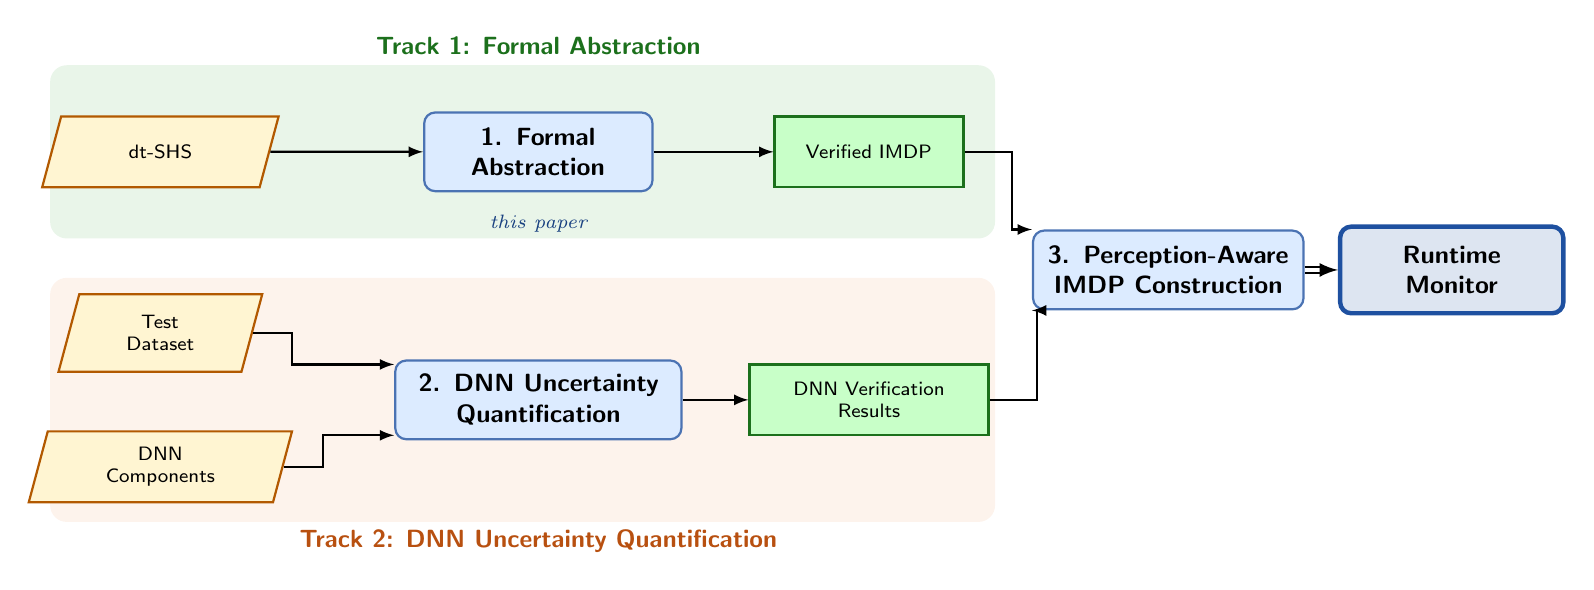
\begin{tikzpicture}[
				pipe_input/.style  = {draw=orange!70!black, trapezium, trapezium left angle=75,
					trapezium right angle=105, thick, minimum width=2.6cm, minimum height=0.9cm,
					align=center, fill=inputYellow, font=\scriptsize\sffamily},
				pipe_proc/.style   = {draw=imdpBlue!80, rectangle, rounded corners=4pt, thick,
					minimum width=2.9cm, minimum height=1.0cm, align=center,
					fill=imdpLightBlue, font=\small\sffamily\bfseries},
				pipe_out/.style    = {draw=safeGreen!70!black, rectangle, thick,
					minimum width=2.4cm, minimum height=0.9cm, align=center,
					fill=outputGreen, font=\scriptsize\sffamily},
				pipe_final/.style  = {draw=imdpBlue, rectangle, rounded corners=4pt, ultra thick,
					minimum width=2.4cm, minimum height=1.1cm, align=center,
					fill=imdpBlue!15, font=\small\sffamily\bfseries},
				line/.style        = {->, thick, >=latex, font=\scriptsize\sffamily}
				]
				\fill[safeGreen!10, rounded corners=6pt] (-1.4, 0.3) rectangle (10.6, 2.5);
				\fill[accentOrange!8, rounded corners=6pt] (-1.4, -3.3) rectangle (10.6, -0.2);
				
				\node[font=\small\sffamily\bfseries, text=safeGreen!70!black]
				at (4.8, 2.75) {Track 1: Formal Abstraction};
				\node[font=\small\sffamily\bfseries, text=accentOrange!80!black]
				at (4.8, -3.55) {Track 2: DNN Uncertainty Quantification};
				
				\node[pipe_input, text width=0.9cm, align=center] (plant_in) at (0, 1.4) {dt-SHS};
				\node[pipe_proc, text width=2.4cm] (disc) at (4.8, 1.4) {1. Formal\\Abstraction};
				\node[pipe_out, text width=1.8cm] (disc_out) at (9.0, 1.4) {Verified IMDP};
				
				\draw[line] (plant_in) -- (disc);
				\draw[line] (disc) -- (disc_out);
				\node[below=0.16cm of disc, font=\itshape\scriptsize\color{imdpBlue!80!black}] {this paper};
				
				\node[pipe_input, text width=1.2cm, align=center] (data) at (0, -0.9) {Test Dataset};
				\node[pipe_input, text width=2.1cm, align=center] (dnn_in) at (0, -2.6) {DNN\\Components};
				
				\node[pipe_proc, text width=3.4cm] (uq) at (4.8, -1.75)
				{2. DNN Uncertainty\\Quantification};
				\node[pipe_out, text width=2.8cm] (uq_out) at (9.0, -1.75)
				{DNN Verification\\Results};
				
				\draw[line] (data.east) -- ++(0.5,0) |- ([yshift=0.45cm]uq.west);
				\draw[line] (dnn_in.east) -- ++(0.5,0) |- ([yshift=-0.45cm]uq.west);
				\draw[line] (uq) -- (uq_out);
				
				\node[pipe_proc, text width=3.2cm] (contracts) at (12.8, -0.1)
				{3. Perception-Aware\\IMDP Construction};
				\draw[line] (disc_out.east) -- ++(0.6,0) |- (contracts.north west);
				\draw[line] (uq_out.east) -- ++(0.6,0) |- (contracts.south west);
				
				\node[pipe_final, text width=2.6cm] (monitor) at (16.4, -0.1)
				{\textbf{Runtime}\\\textbf{Monitor}};
				\draw[line, double, double distance=1.5pt] (contracts) -- (monitor);
			\end{tikzpicture}%
		}
		\caption{Building blocks of the wider verification programme. This paper documents Track~1.}
		\label{fig:programme}
	\end{figure}
	
	The remainder of the paper is organised as follows. Section~\ref{sec:bg} fixes terminology, recalls the probabilistic invariance problem, and states the robust-verification framework on which soundness rests. Section~\ref{sec:rw} positions the work relative to the partition-based abstraction literature. Section~\ref{sec:abs} presents the abstraction procedure and the soundness analysis in detail. Section~\ref{sec:cs} develops the AEBS case study and reports the certificates and the verification campaigns. Section~\ref{sec:concl} concludes.
	
	\section{Background}
	\label{sec:bg}
	
	This section fixes the class of system models we abstract from, the class of finite-state models we abstract to, the verification question we wish to answer, and the framework under which a containing IMDP is a sound surrogate for the continuous system.
	
	\subsection{Discrete-time stochastic hybrid systems}
	\label{sec:bg:dtshs}
	
	Following the formalisation of~\cite[Def.~1.2]{LSAZ22}, a \emph{discrete-time stochastic hybrid system} (dt-SHS) is a tuple
	\begin{equation}
		\Sigma \;=\; (Q,\; n,\; X,\; U,\; T_x,\; Y,\; h),
		\label{eq:dtshs}
	\end{equation}
	where $Q = \{q_1, \ldots, q_p\}$ is a finite set of discrete modes; $n : Q \to \mathbb{N}_{\ge 1}$ assigns to each mode a continuous-state dimension; $X \subseteq \bigcup_{q \in Q} \{q\} \times \R^{n(q)}$ is the hybrid state space with Borel $\sigma$-algebra $\mathcal{B}(X)$; $U \subseteq \R^m$ is a Borel input space; $T_x : \mathcal{B}(X) \times X \times U \to [0,1]$ is a conditional stochastic kernel; $Y$ is a Borel output space; and $h : X \to Y$ is a measurable output map. The kernel $T_x$ characterises the one-step transition law: for any $A \in \mathcal{B}(X)$ and any $k \in \mathbb{N}$,
	\begin{equation}
		\Prob\bigl(x(k+1) \in A \,\big|\, x(k), \nu(k)\bigr) \;=\; \int_A T_x\bigl(dx(k+1) \,\big|\, x(k), \nu(k)\bigr),
		\label{eq:dtshs-kernel}
	\end{equation}
	where $x(k) \in X$ is the state at step $k$ and $\nu(k) \in U$ is the input applied at that step.
	
	When $|Q| = 1$ the discrete component is trivial and the model reduces to a discrete-time stochastic control system over a continuous state space~\cite[Def.~1.3]{LSAZ22}; this is the form taken by the case study of Section~\ref{sec:cs}.
	
	\subsection{Interval Markov decision processes}
	\label{sec:bg:imdp}
	
	The target of the abstraction is a finite-state model with interval-valued transition probabilities. Following~\cite{GLD00}, an \emph{Interval Markov Decision Process} (IMDP, also called a \emph{bounded-parameter MDP}) is a tuple
	\begin{equation}
		\mathcal{I} \;=\; (\hat S,\; \hat U,\; \check P,\; \hat P),
		\label{eq:imdp}
	\end{equation}
	where $\hat S$ is a finite set of states, $\hat U$ a finite set of actions, and $\check P, \hat P : \hat S \times \hat U \times \hat S \to [0,1]$ are lower- and upper-bound transition functions with $\check P(s,a,s') \le \hat P(s,a,s')$ for every triple. The IMDP represents the set of all MDPs whose exact transition probabilities $P(s,a,s')$ satisfy $\check P(s,a,s') \le P(s,a,s') \le \hat P(s,a,s')$ and whose rows sum to one. Verification of an IMDP property is performed against the worst-case (or, dually, best-case) choice of transition distribution consistent with the stored intervals, so the output is itself an interval bracketing the property value over the entire set of consistent MDPs.
	
	\subsection{The probabilistic invariance problem}
	\label{sec:bg:inv}
	
	For a dt-SHS $\Sigma$ with state space $X$, the \emph{probabilistic invariance} (finite-horizon safety) problem~\cite{APLS08} is to compute, for each initial state $x_0 \in X$, the probability
	\begin{equation}
		p_{x_0}(A) \;=\; \Prob\bigl(\,x(k) \in A\ \text{for all } k \in [0, N] \,\big|\, x(0) = x_0\,\bigr),
		\label{eq:invariance}
	\end{equation}
	where $A \subseteq X$ is the Borel set of safe states, $N$ a finite horizon, and $x(k)$ the state under the kernel $T_x$. The quantity in~\eqref{eq:invariance} can be characterised as the value at time $0$ of a backward Bellman recursion over $A$~\cite[Thm.~1]{APLS08}; the recursion involves integrals against $T_x$ that are generally intractable in closed form, which motivates a finite-state abstraction on which the discrete analogue of the recursion is computable.
	
	\subsection{Robust verification of interval models}
	\label{sec:bg:robust}
	
	An IMDP denotes a \emph{set} of Markov decision processes, namely all those whose row-stochastic transition probabilities lie within the stored intervals. This is the object studied under the name \emph{Markov set-chain}~\cite{Hartfiel98}. Robust verification of a temporal-logic property over an IMDP computes the extremal value of the property over the whole denoted set. The preservation result we rely on is that of~\cite{DAK12}: when one model's transition probabilities are contained, transition by transition, within the intervals of an interval model, the robust PCTL value computed on the interval model brackets the property value of the contained model. Containment of the concrete transition probabilities within the abstract intervals is therefore the single hypothesis under which a verification result on the IMDP transfers to the system being abstracted; the notion of approximate abstraction for stochastic hybrid systems we use originates with~\cite{ADD11}. We make this hypothesis precise and discharge it in Section~\ref{sec:abs:sound}.
	
	\section{Related Work}
	\label{sec:rw}
	
	Automated verification and synthesis of stochastic hybrid systems is a broad and active area, surveyed recently by~\cite{LSAZ22}; partition-based finite abstraction is one approach within it, and the one to which our work belongs. That survey also identifies the compositional construction of interval Markov processes as one of its open problems. Two prior constructions are most relevant to ours. The first,~\cite{ADD11}, introduces approximate abstractions of stochastic hybrid systems: the continuous state space is partitioned, a finite Markov model is built over the cells, and the abstraction is accompanied by an a priori bound on the difference between the abstract and concrete probabilistic-safety values, governed by the regularity of the stochastic kernel and the resolution of the partition. The second,~\cite{Soudjani2013}, develops adaptive and sequential gridding procedures for the same setting: it refines the partition where the kernel varies most rather than uniformly, and supplies a per-transition range bound (its Equation~3.11), which measures the kernel's actual variation over a source cell, alongside an additive global error bound that accumulates over the verification horizon and that the refinement is designed to reduce. As that procedure makes explicit, adaptive refinement helps most when the per-cell error is spatially non-uniform, so that resolution can be concentrated where it most reduces the global bound.
	
	The construction documented here is also a partition-based abstraction for a stochastic hybrid system with a finite action set, but it targets an interval-valued model and certifies soundness by per-transition containment rather than by an analytic global bound. From~\cite{Soudjani2013} it reuses a single analytic ingredient, the per-transition range bound of Equation~3.11, applied at the integrated-kernel level on the one stochastic dimension; it adopts neither the adaptive gridding nor the additive global bound as a soundness mechanism. The reason is twofold. First, structurally: the AEBS kernel is degenerate, a product of Dirac point masses on the deterministic dimensions and a single Gaussian, so it admits no density on the full state space. The error analysis of~\cite{Soudjani2013} rests on Lipschitz continuity of the conditional density, an assumption that line of work states explicitly and that its benchmark systems satisfy by carrying full-support noise on every continuous state variable~\cite{SGA15,SAM15}; on the deterministic dimensions here, the cell-to-cell probability is an indicator that jumps between $0$ and $1$, which no finite Lipschitz constant describes, so the additive bound is inapplicable there rather than merely loose. Second, quantitatively: on the one dimension where a density does exist, the noise is constant, so the per-row interval width is essentially uniform across the state space, which leaves the adaptive procedure no heterogeneity to exploit and renders the additive bound uninformative at practical horizons; this second obstacle would persist even under full-support constant noise. Degenerate noise of this kind is addressed in a more recent branch of the same literature, which likewise reaches for interval-valued models certified by per-transition bounds: \cite{SLFL23} abstracts systems $x^{+} = f(x, w)$ whose noise domain has dimension decoupled from the state's, by partitioning the noise domain and bounding each transition through set-valued images, and \cite{DC18,DHC22} combine mixed-monotone reachable-set computation on the deterministic dynamics with interval-valued transition bounds. Our construction belongs to this interval branch while retaining the per-transition range bound of~\cite{Soudjani2013} on the dimension where its density premise holds. Soundness is obtained instead from per-transition containment under the Markov set-chain preservation result~\cite{DAK12,Hartfiel98}, in the approximate-abstraction sense of~\cite{ADD11}, with the additive bound retained only as a diagnostic. The handling of the deterministic dimensions and the full rationale are developed where they arise (Sections~\ref{sec:abs:intervals} and~\ref{sec:abs:rel}). The choice of an interval-valued target model is motivated, as in Section~\ref{sec:intro}, by the need to carry both partition-induced and perception-induced uncertainty through to the verifier.
	
	\section{The Abstraction Procedure}
	\label{sec:abs}
	
	This section presents the construction. Section~\ref{sec:abs:partition} partitions the continuous state space into the states of the IMDP; Section~\ref{sec:abs:intervals} computes the probability intervals attached to its transitions; Section~\ref{sec:abs:sound} establishes soundness through the containment certificate, the exhaustive per-transition test by which the IMDP is proved to over-approximate the continuous system; Section~\ref{sec:abs:full} composes the steps into the end-to-end pipeline that emits the abstraction for the verifier.
	
	The procedure applies to the following class of systems, which mixes
	deterministic and stochastic state variables; the two kinds of dimension
	are treated by different mechanisms at every stage of the construction.
	
	\begin{assumption}[System class]\phantomsection\label{ass:sysclass}
		The system is a dt-SHS~\eqref{eq:dtshs} with $|Q| = 1$, so that the
		hybrid state reduces to the continuous state $s \in \mathcal{S}$, with
		$\mathcal{S} \subseteq \R^n$ bounded and the action set $U$ finite. For
		every action $a \in U$:
		\begin{enumerate}[label=(\roman*)]
			\item \emph{Additive independent noise.} One step from state $s$ under
			action $a$ lands at
			\begin{equation}
				s' \;=\; \mu(s, a) + w,
				\label{eq:addnoise}
			\end{equation}
			where
			\begin{itemize}
				\item $s' \in \R^n$ is the successor state;
				\item $\mu : \mathcal{S} \times U \to \R^n$ is the one-step mean map,
				giving the successor before noise;
				\item $w \in \R^n$ is the noise vector; its components $w_d$ are
				independent of one another. In each \emph{deterministic} dimension,
				$w_d = 0$, written $\sigma_d = 0$. In each \emph{stochastic} dimension,
				$w_d$ follows the normal distribution with mean zero and variance
				$\sigma_d^2$, written $w_d \sim \Norm(0, \sigma_d^2)$, where the
				standard deviation $\sigma_d > 0$ is constant over $\mathcal{S}$.
			\end{itemize}
			Equivalently, the one-step kernel factorises across the dimensions,
			\begin{equation}
				T_x\bigl(A_1 \times \dots \times A_n \mid s, a\bigr)
				\;=\; \prod_{d=1}^{n} T_{x,d}\bigl(A_d \mid s, a\bigr),
				\label{eq:kernelfactor}
			\end{equation}
			where
			\begin{itemize}
				\item $T_x$ is the one-step kernel of~\eqref{eq:dtshs-kernel};\item $A_d \subseteq \R$ is an interval of values for coordinate $d$
				of the successor state;
				\item $A_1 \times \dots \times A_n$ is the region of states that meet
				all $n$ of these interval conditions at once, one per coordinate;
				\item $T_{x,d}(A_d \mid s, a)$ is the probability that coordinate $d$
				of the successor state falls in $A_d$. In a deterministic dimension
				the coordinate is exactly $\mu_d(s, a)$, so this probability is $1$
				if $\mu_d(s, a)$ lies in $A_d$ and $0$ if it does not. In a stochastic
				dimension the coordinate is $\mu_d(s, a)$ plus the noise $w_d$, so it
				is the probability that this noisy value lands in $A_d$.
			\end{itemize}
			\item \emph{Continuity.} The map $s \mapsto \mu(s, a)$ is continuous on
			$\mathcal{S}$.
			
			\item \emph{Component-wise monotonicity.} Take any one coordinate of
			the state and change it upward, keeping the rest of the state as it
			is. Each coordinate of $\mu(s, a)$ then responds in a fixed way: it
			only ever rises (or stays put), or it only ever falls (or stays put).
			Which of the two happens depends on the pair of coordinates involved,
			but never on where in $\mathcal{S}$ the change is made.
			
		\end{enumerate}
	\end{assumption}
	
	The additive form~\eqref{eq:addnoise} is the standard shape in this
	abstraction literature~\cite{Soudjani2013}; the component-wise
	monotonicity of part~(iii) is the property exploited for corner-based
	reachable-set computation in~\cite{CA15}; the mixed Dirac and Gaussian
	split is the restriction this construction is designed for. That the
	case study satisfies the assumption is established in
	Section~\ref{sec:cs}; the constancy of $\sigma_d$ in part~(i) is
	additionally checked at construction time (Algorithm~\ref{alg:imagebox}).
	
	\subsection{Partitioning the state space}
	\label{sec:abs:partition}
	
	Following the partition-based abstraction approach
	of~\cite{ADD11,Soudjani2013}, the continuous state space is covered by
	a finite grid of non-overlapping cells. Terminology is fixed as
	follows; Figure~\ref{fig:cellstate} depicts the three notions. The
	space $\mathcal{S}$ belongs entirely to the concrete system, and a
	\emph{continuous state} is a point of $\mathcal{S}$. A \emph{cell} is
	a region of $\mathcal{S}$ delimited by the grid. A \emph{state} is an
	element of the finite model and carries no geometry of its own. The
	two sides are connected by mapping each cell to one state. The finite
	model occupying state $i$ means that the concrete system lies at some
	point of the cell $A_i$, with no record of which; the transition
	intervals of Section~\ref{sec:abs:intervals} are constructed to be
	valid for every such point.
	
	\begin{figure}[h]
		\centering
		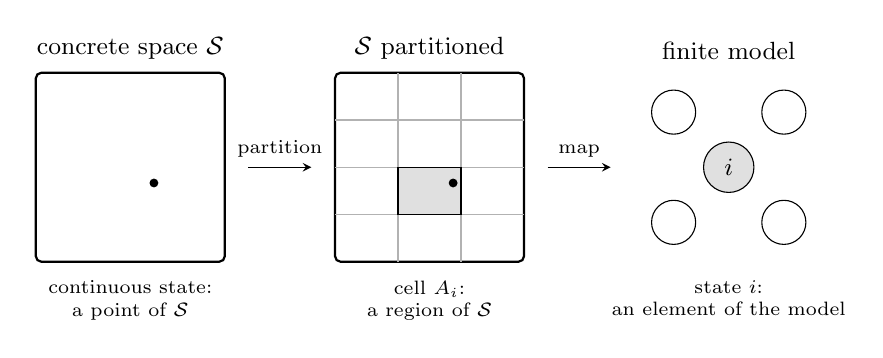
\begin{tikzpicture}[>=stealth, font=\small]
			\draw[rounded corners=2pt, thick] (0,0) rectangle (2.4,2.4);
			\node[anchor=south] at (1.2,2.45) {concrete space $\mathcal{S}$};
			\fill (1.5,1.0) circle (1.6pt);
			\node[anchor=north, font=\scriptsize, align=center] at (1.2,-0.12)
			{continuous state:\\ a point of $\mathcal{S}$};
			\draw[->] (2.7,1.2) -- (3.5,1.2)
			node[midway, above, font=\scriptsize] {partition};
			\begin{scope}[shift={(3.8,0)}]
				\draw[rounded corners=2pt, thick] (0,0) rectangle (2.4,2.4);
				\foreach \x in {0.8,1.6} \draw[gray!60, thin] (\x,0) -- (\x,2.4);
				\foreach \y in {0.6,1.2,1.8} \draw[gray!60, thin] (0,\y) -- (2.4,\y);
				\fill[black!12] (0.8,0.6) rectangle (1.6,1.2);
				\draw (0.8,0.6) rectangle (1.6,1.2);
				\fill (1.5,1.0) circle (1.6pt);
				\node[anchor=south] at (1.2,2.45) {$\mathcal{S}$ partitioned};
				\node[anchor=north, font=\scriptsize, align=center] at (1.2,-0.12)
				{cell $A_i$:\\ a region of $\mathcal{S}$};
			\end{scope}
			\draw[->] (6.5,1.2) -- (7.3,1.2)
			node[midway, above, font=\scriptsize] {map};
			\begin{scope}[shift={(7.6,0)}]
				\node[anchor=south] at (1.2,2.45) {finite model};
				\foreach \p in {(0.5,1.9),(1.9,1.9),(0.5,0.5),(1.9,0.5)}
				\draw \p circle (0.28);
				\draw[fill=black!12] (1.2,1.2) circle (0.32);
				\node at (1.2,1.2) {$i$};
				\node[anchor=north, font=\scriptsize, align=center] at (1.2,-0.12)
				{state $i$:\\ an element of the model};
			\end{scope}
		\end{tikzpicture}
		\caption{Continuous states, cells, and states. Left: a continuous
			state is a point of the concrete space $\mathcal{S}$. Centre: the
			partition delimits cells; the point has not moved and lies in cell
			$A_i$. Right: a state is an element of the finite model; cell
			$A_i$ is mapped to state $i$.}
		\label{fig:cellstate}
	\end{figure}
	
	The complete state set of the model, including its absorbing states,
	is assembled at the end of this subsection. The bounded state space is
	covered as
	\begin{equation}
		\mathcal{S} \;\subseteq\; \bigcup_{i=1}^{M} A_i, \qquad
		A_i \cap A_j = \emptyset \ \ \text{for } i \neq j,
		\label{eq:partition}
	\end{equation}
	where
	\begin{itemize}
		\item $\mathcal{S} \subseteq \R^n$ is the continuous state space;
		\item $A_i$ is the $i$-th cell, a bounded region of $\mathcal{S}$
		containing uncountably many continuous states;
		\item $M$ is the total number of cells.
	\end{itemize}
	
	The coordinates of $\mathcal{S}$ are indexed $d = 1, \dots, n$ and
	called \emph{dimensions}. Each cell is specified by one interval of
	values per dimension and contains exactly the continuous states whose
	coordinate in each dimension lies in that dimension's interval; a
	region of this form is called an \emph{axis-aligned box}, and
	Figure~\ref{fig:cellgeom} shows one cell with its defining intervals. \newline
	Each interval is \emph{half-open}, containing its lower endpoint and
	excluding its upper endpoint,
	\begin{equation}
		A_i \;=\; \prod_{d=1}^{n} \bigl[\, \mathrm{lo}_{i,d},\ \mathrm{hi}_{i,d} \,\bigr),
		\label{eq:cellbox}
	\end{equation}
	where
	\begin{itemize}
		\item $\mathrm{lo}_{i,d}$ and $\mathrm{hi}_{i,d}$ are the lower and
		upper endpoints of cell $i$'s interval in dimension $d$.
	\end{itemize}
	
	\begin{figure}[h]
		\centering
		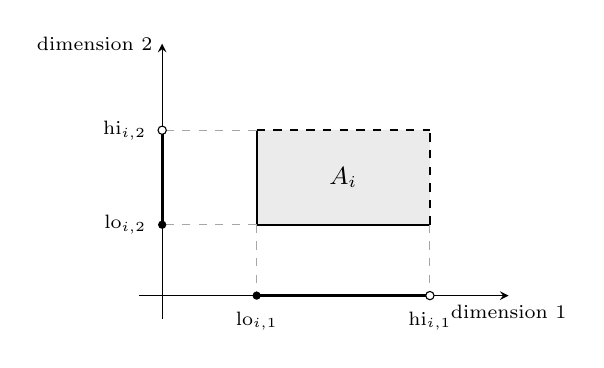
\begin{tikzpicture}[>=stealth, font=\small]
			\draw[->] (-0.3,0) -- (4.4,0) node[below] {\scriptsize dimension $1$};
			\draw[->] (0,-0.3) -- (0,3.2) node[left] {\scriptsize dimension $2$};
			\fill[black!8] (1.2,0.9) rectangle (3.4,2.1);
			\draw[thick] (1.2,0.9) -- (3.4,0.9);
			\draw[thick] (1.2,0.9) -- (1.2,2.1);
			\draw[thick, dashed] (3.4,0.9) -- (3.4,2.1);
			\draw[thick, dashed] (1.2,2.1) -- (3.4,2.1);
			\node at (2.3,1.5) {$A_i$};
			\draw[gray!70, thin, dashed] (1.2,0.9) -- (1.2,0);
			\draw[gray!70, thin, dashed] (3.4,0.9) -- (3.4,0);
			\draw[very thick] (1.2,0) -- (3.4,0);
			\fill (1.2,0) circle (1.5pt);
			\draw[fill=white] (3.4,0) circle (1.5pt);
			\node[below, font=\scriptsize] at (1.2,-0.08) {$\mathrm{lo}_{i,1}$};
			\node[below, font=\scriptsize] at (3.4,-0.08) {$\mathrm{hi}_{i,1}$};
			\draw[gray!70, thin, dashed] (1.2,0.9) -- (0,0.9);
			\draw[gray!70, thin, dashed] (1.2,2.1) -- (0,2.1);
			\draw[very thick] (0,0.9) -- (0,2.1);
			\fill (0,0.9) circle (1.5pt);
			\draw[fill=white] (0,2.1) circle (1.5pt);
			\node[left, font=\scriptsize] at (-0.08,0.9) {$\mathrm{lo}_{i,2}$};
			\node[left, font=\scriptsize] at (-0.08,2.1) {$\mathrm{hi}_{i,2}$};
		\end{tikzpicture}
		\caption{One cell and its defining intervals, drawn for $n = 2$. The
			cell $A_i$ contains exactly the continuous states whose coordinate in
			each dimension lies in that dimension's interval. Solid edges belong
			to the cell and dashed edges do not: each interval contains its lower
			endpoint (filled) and excludes its upper endpoint (open).}
		\label{fig:cellgeom}
	\end{figure}
	
	A point lying on a boundary shared by two cells therefore belongs to
	exactly one of them, the cell whose lower endpoint it is. This is what
	makes the cells of~\eqref{eq:partition} pairwise disjoint while
	covering $\mathcal{S}$: every continuous state lies in exactly one
	cell.
	
	The grid is uniform: in each dimension $d$, all cells have the same
	width $r_d$, the grid \emph{resolution} in that dimension. The cells
	of a dimension are delimited by a sorted list of boundary values, its
	\emph{edges}: the first cell lies between the first and second edge,
	the second cell between the second and third, and so on, as
	Figure~\ref{fig:edges} shows. The edges of dimension $d$ are
	\begin{equation}
		\text{edges}_d \;=\; \Bigl(\, \ell_d - \tfrac{r_d}{2},\;
		\ell_d + \tfrac{r_d}{2},\; \ell_d + \tfrac{3 r_d}{2},\; \dots,\;
		h_d + \tfrac{r_d}{2} \,\Bigr),
		\label{eq:bins}
	\end{equation}
	where
	\begin{itemize}
		\item $r_d$ is the resolution in dimension $d$;
		\item $\ell_d$ and $h_d$ are the lower and upper bounds of dimension
		$d$;
		\item $\text{edges}_d$ is the resulting list: it starts half a cell
		below $\ell_d$ and advances in steps of $r_d$ until half a cell above
		$h_d$.
	\end{itemize}
	
	\begin{figure}[h]
		\centering
		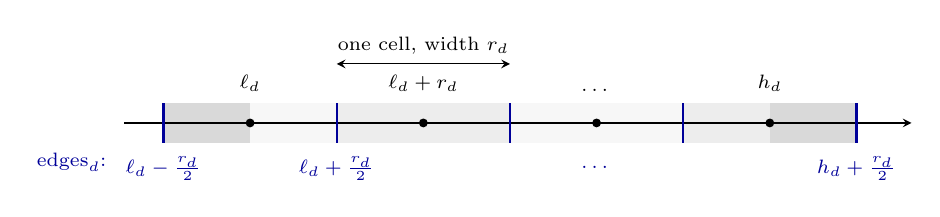
\begin{tikzpicture}[>=stealth, font=\small]
			% cells as alternating strips (band height 0.5)
			\fill[gray!6]  (0.4,-0.25) rectangle (2.6,0.25);
			\fill[gray!14] (2.6,-0.25) rectangle (4.8,0.25);
			\fill[gray!6]  (4.8,-0.25) rectangle (7.0,0.25);
			\fill[gray!14] (7.0,-0.25) rectangle (9.2,0.25);
			% overhang halves, darker
			\fill[gray!30] (0.4,-0.25) rectangle (1.5,0.25);
			\fill[gray!30] (8.1,-0.25) rectangle (9.2,0.25);
			% axis
			\draw[->] (-0.1,0) -- (9.9,0);
			% edges: blue ticks spanning the band
			\foreach \x in {0.4,2.6,4.8,7.0,9.2}
			\draw[thick, blue!60!black] (\x,-0.25) -- (\x,0.25);
			\node[anchor=east, font=\scriptsize, blue!60!black] at (-0.2,-0.5)
			{$\text{edges}_d$:};
			\node[below, font=\scriptsize, blue!60!black] at (0.4,-0.3)
			{$\ell_d - \tfrac{r_d}{2}$};
			\node[below, font=\scriptsize, blue!60!black] at (2.6,-0.3)
			{$\ell_d + \tfrac{r_d}{2}$};
			\node[below, font=\scriptsize, blue!60!black] at (5.9,-0.42) {$\dots$};
			\node[below, font=\scriptsize, blue!60!black] at (9.2,-0.3)
			{$h_d + \tfrac{r_d}{2}$};
			% centres: black dots, labels above
			\foreach \x in {1.5,3.7,5.9,8.1} \fill (\x,0) circle (1.6pt);
			\node[above, font=\scriptsize] at (1.5,0.28) {$\ell_d$};
			\node[above, font=\scriptsize] at (3.7,0.28) {$\ell_d + r_d$};
			\node[above, font=\scriptsize] at (5.9,0.28) {$\dots$};
			\node[above, font=\scriptsize] at (8.1,0.28) {$h_d$};
			% one cell width, marked across the second strip
			\draw[<->] (2.6,0.75) -- (4.8,0.75)
			node[midway, above, font=\scriptsize] {one cell, width $r_d$};
		\end{tikzpicture}
		\caption{The edges of one dimension, drawn for four cells. The blue
			ticks are the entries of $\text{edges}_d$ in~\eqref{eq:bins}; each
			pair of consecutive edges delimits one cell, shown as alternating
			strips of width $r_d$. The black points are the cell centres. The
			first edge sits half a cell below the lower bound $\ell_d$, so the
			bounds $\ell_d$ and $h_d$ fall on the centres of the outermost cells;
			the darker strips are the halves of those cells extending beyond the
			bounds.}
		\label{fig:edges}
	\end{figure}
	
	Placing the values $\ell_d,\ \ell_d + r_d,\ \dots,\ h_d$ in cell
	interiors rather than on cell boundaries has two effects:
	floating-point rounding of a value computed at such a continuous
	state cannot move it across a cell boundary, and the centre of a cell
	can coincide exactly with the continuous state it represents. Because
	the outermost cells extend half a cell beyond the bounds, the union
	of the cells strictly contains $\mathcal{S}$;
	\eqref{eq:partition} therefore states a covering rather than an
	equality.
	
	
	
	Writing $n_d$ for the number of cells along dimension $d$, the grid total cells are described as follows 
	\begin{equation}
		M \;=\; \prod_{d=1}^{n} n_d
		\label{eq:Mcount}
	\end{equation}
	
	
	Each cell is assigned one integer state identifier. The cells are
	enumerated in \emph{row-major order}, the convention in which the
	index of the last dimension varies fastest, and the per-dimension
	cell indices $(k_1, \dots, k_n)$ are flattened into a single integer.
	Distinct index tuples receive distinct identifiers, and each
	identifier corresponds to exactly one cell. The centre $c_i$ of each
	cell is recorded alongside it. The centre plays no role in the
	transition construction of Section~\ref{sec:abs:intervals}, which
	bounds the dynamics over every continuous state of a cell rather than
	at any single representative point; it is the evaluation point of the
	\hyperref[par:labelling]{state labelling}.\newline
	
	\phantomsection\label{par:labelling}%
	The questions later posed to the model concern regions of the
	state space, and a \emph{label} is a name attached to states so
	that such a region becomes addressable. A label is defined by a
	\emph{predicate}, a yes-or-no condition on the continuous state.
	The predicate may involve any dimensions and any quantity computed
	from them, and a state may carry several labels at once. A state
	receives a label exactly when the label's predicate holds at the
	centre of the state's cell. A cell that contains continuous states
	on both sides of a predicate's boundary is therefore labelled by
	its centre's answer throughout its extent, so what the labels
	describe is the predicate as quantised on the grid; refining the
	grid shrinks the cells on which the two disagree.\newline
	
	The model contains \emph{absorbing} states of two kinds. A state is
	absorbing when, under every action, its only transition is the
	certain self-loop $[1,1]$ to itself: a run that enters an absorbing
	state remains there. The first kind handles a designated
	\emph{terminal region} of $\mathcal{S}$: the region of a label whose
	outcome is decided at entry, meaning the property under study is
	settled the moment a run first satisfies the label's predicate, so
	the dynamics need not be tracked further. One grid cell inside the
	region is designated its representative and made absorbing, and the
	interval construction of Section~\ref{sec:abs:intervals} routes to
	the representative every transition whose reachable set meets the
	region; a terminal region therefore introduces no state beyond the
	$M$ grid cells. The construction designates a single terminal
	region, as the case study of Section~\ref{sec:cs} has one outcome
	decided at entry; further such regions would be handled identically,
	each through its own absorbing representative and label. The second
	kind is the \emph{safe sink}, one additional state appended after
	the $M$ grid cells. The dynamics are not confined to the modelled
	window $\mathcal{S}$, and the sink receives the probability mass of
	transitions that leave the grid. The kinds carry distinct labels for
	the verifier: mass absorbed at a terminal representative bears on
	the property being checked, whereas mass in the sink records
	departure from the modelled window, and separate labels keep the
	contributions separately quantifiable. \newline
	
	The construction also records a \emph{partition fingerprint}, a hash
	of the exact edge values of every dimension; two runs operate on the
	same partition exactly when their fingerprints match.
	
	Algorithm~\ref{alg:grid} records this partitioning step: it lays down
	the cell edges of~\eqref{eq:bins} in each dimension, enumerates the
	Cartesian product of cell indices in row-major order, attaches the
	labels at cell centres, designates the terminal-region
	representative, and appends the safe sink.
	
	\begin{algorithm}[H]
		\caption{Grid construction.}
		\label{alg:grid}
		\begin{algorithmic}[1]
			\Require bounds $(\ell_d, h_d)$ and resolution $r_d$ per
			dimension; labelling predicates; terminal region
			\Ensure partition $\{A_i\}_{i=1}^M$, identifiers, centres,
			fingerprint, labels, designated absorbing states
			\State per dimension, compute the cell count and set
			$\text{edges}_d$~\eqref{eq:bins}
			\State enumerate cells; assign row-major identifiers
			\State record cell centres and the partition fingerprint
			\State attach to each state the labels whose predicates hold
			at its cell's centre
			\State designate the terminal representative; reserve the sink
			identifier
			\State \Return partition, identifiers, centres, fingerprint,
			labels, absorbing states
		\end{algorithmic}
	\end{algorithm}
	
	
	\subsection{Per-transition probability intervals}
	\label{sec:abs:intervals}
	
	Each cell $A_i$ of Section~\ref{sec:abs:partition} corresponds to one state, and both are indexed by $i$. Transitions of the IMDP connect states, but the one-step law of the concrete system acts on the continuous states inside the cells: for a fixed action $a \in U$ and target cell $A_j$, the one-step probability
	\begin{equation}
		T_x(A_j \mid s, a), \qquad s \in A_i,
		\label{eq:txonstates}
	\end{equation}
	is a function of the source state $s$ and generally takes different values across the cell, while the IMDP carries a single transition from state $i$ to state $j$. The construction therefore stores, for each non-absorbing source cell $A_i$, each action $a \in U$, and each reachable target cell $A_j$, an interval $[p_{\min}, p_{\max}]$ satisfying
	\begin{equation}
		p_{\min} \;\le\; T_x(A_j \mid s, a) \;\le\; p_{\max} \qquad \text{for every } s \in A_i.
		\label{eq:cellcontain}
	\end{equation}
	This uniform containment over the source cell is the hypothesis under which verification results transfer from the IMDP to the continuous system~\cite{DAK12} (Section~\ref{sec:abs:sound}). The interval for a transition is built in three steps. First, bound the region that the dynamics can send the source cell to; this bound is the \emph{image box}. Second, for each dimension, bracket the probability that the successor's coordinate lands in the target cell's interval; the deterministic and stochastic dimensions of \hyperref[ass:sysclass]{Assumption~(i)} are bracketed by separate mechanisms. Third, multiply the per-dimension brackets, which by the factorisation~\eqref{eq:kernelfactor} brackets the transition probability itself.
	
	\paragraph{The image box.}
	By \hyperref[ass:sysclass]{Assumption~(i)}, a step from $s$ under $a$ lands at the mean point $\mu(s, a)$ plus the per-dimension noise $w$. Applying the mean map to every state of the source cell gives the \emph{image set}
	\begin{equation}
		\mu(A_i, a) \;=\; \{\, \mu(s, a) : s \in A_i \,\},
		\label{eq:imageset}
	\end{equation}
	the set of mean points to which the cell's states are sent (Figure~\ref{fig:imagebox}). The image set is in general not aligned to the grid and consists of uncountably many points, so it is not enumerated directly. The construction encloses it in the smallest axis-aligned box that contains it, the \emph{image box}
	\begin{equation}
		B_i^a \;=\; \prod_{d=1}^{n} \bigl[\, \mu_d^{\text{lo}},\ \mu_d^{\text{hi}} \,\bigr],
		\label{eq:imageboxdef}
	\end{equation}
	where
	\begin{itemize}
		\item $B_i^a$ is the image box of source cell $A_i$ under action $a$;
		\item $\mu_d^{\text{lo}}$ and $\mu_d^{\text{hi}}$ are the smallest and largest values that coordinate $d$ of the mean $\mu(s, a)$ takes as $s$ ranges over the cell $A_i$.
	\end{itemize}
	The box contains the image set, so any transition bound computed against the box holds for every continuous state of the cell; and it is a product of one-dimensional intervals, which is the form the per-dimension factorisation of~\eqref{eq:kernelfactor} requires.
	
	Computing $\mu_d^{\text{lo}}$ and $\mu_d^{\text{hi}}$ directly would
	mean searching over the uncountably many continuous states of the
	cell. Component-wise monotonicity
	(\hyperref[ass:sysclass]{Assumption~(iii)}) removes that search. In
	one dimension the principle is elementary: a monotone function on an
	interval attains its smallest and largest values at the interval's
	two ends. Extending this to a cell requires the cell's counterpart of
	the interval ends. The cell $A_i$ has one interval per
	dimension~\eqref{eq:cellbox}; the interval in dimension $d$ runs from
	$\mathrm{lo}_{i,d}$ to $\mathrm{hi}_{i,d}$, and these two values are
	its \emph{endpoints}. A \emph{corner} of the cell is a point whose
	coordinate in every dimension is one of that dimension's two
	endpoints. Figure~\ref{fig:corners} shows the four corners of a
	two-dimensional cell, each labelled by the pair of endpoints that
	builds it; with two possible endpoints in each of $n$ dimensions, a
	cell has $2^n$ corners.
	
	\begin{figure}[h]
		\centering
		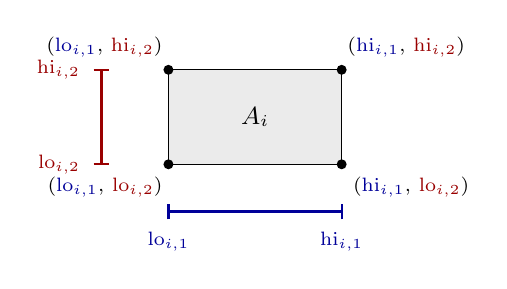
\begin{tikzpicture}[>=stealth, font=\small]
			\draw[very thick, blue!60!black] (1.2,0.3) -- (3.4,0.3);
			\draw[thick, blue!60!black] (1.2,0.2) -- (1.2,0.4);
			\draw[thick, blue!60!black] (3.4,0.2) -- (3.4,0.4);
			\node[below, font=\scriptsize, blue!60!black] at (1.2,0.16) {$\mathrm{lo}_{i,1}$};
			\node[below, font=\scriptsize, blue!60!black] at (3.4,0.16) {$\mathrm{hi}_{i,1}$};
			\draw[very thick, red!60!black] (0.35,0.9) -- (0.35,2.1);
			\draw[thick, red!60!black] (0.25,0.9) -- (0.45,0.9);
			\draw[thick, red!60!black] (0.25,2.1) -- (0.45,2.1);
			\node[left, font=\scriptsize, red!60!black] at (0.2,0.9) {$\mathrm{lo}_{i,2}$};
			\node[left, font=\scriptsize, red!60!black] at (0.2,2.1) {$\mathrm{hi}_{i,2}$};
			\fill[black!8] (1.2,0.9) rectangle (3.4,2.1);
			\draw (1.2,0.9) rectangle (3.4,2.1);
			\node at (2.3,1.5) {$A_i$};
			\foreach \x/\y in {1.2/0.9, 3.4/0.9, 1.2/2.1, 3.4/2.1}
			\fill (\x,\y) circle (1.8pt);
			\node[above left, font=\scriptsize] at (1.25,2.14)
			{$(\textcolor{blue!60!black}{\mathrm{lo}_{i,1}},\, \textcolor{red!60!black}{\mathrm{hi}_{i,2}})$};
			\node[above right, font=\scriptsize] at (3.35,2.14)
			{$(\textcolor{blue!60!black}{\mathrm{hi}_{i,1}},\, \textcolor{red!60!black}{\mathrm{hi}_{i,2}})$};
			\node[below right, font=\scriptsize] at (3.42,0.86)
			{$(\textcolor{blue!60!black}{\mathrm{hi}_{i,1}},\, \textcolor{red!60!black}{\mathrm{lo}_{i,2}})$};
			\node[below left, font=\scriptsize] at (1.25,0.86)
			{$(\textcolor{blue!60!black}{\mathrm{lo}_{i,1}},\, \textcolor{red!60!black}{\mathrm{lo}_{i,2}})$};
		\end{tikzpicture}
		\caption{The corners of a cell, for $n = 2$. The cell's interval in
			dimension $1$ (blue, below) has the two endpoints
			$\mathrm{lo}_{i,1}$ and $\mathrm{hi}_{i,1}$; its interval in
			dimension $2$ (red, left) has the endpoints $\mathrm{lo}_{i,2}$ and
			$\mathrm{hi}_{i,2}$. Each corner pairs one blue endpoint with one red
			endpoint, as its label shows; two choices per dimension give
			$2^n = 4$ corners.}
		\label{fig:corners}
	\end{figure}
	
	Consider one coordinate of the next-state mean $\mu(s, a)$. By
	\hyperref[ass:sysclass]{Assumption~(iii)}, raising any one
	coordinate of the current state $s$ moves it in one fixed direction.
	To make the chosen coordinate of $\mu$ as large as possible over the
	cell, set each coordinate of $s$ to whichever of its two endpoints
	moves it upward; the point built from those choices is, by
	construction, a corner. The smallest value arises in the same way
	with the opposite choices. Both extreme values are therefore found
	among the corner evaluations, so scanning all $2^n$ corners finds
	them without needing to know which direction any coordinate moves:
	\begin{equation}
		[\mu_d^{\text{lo}},\ \mu_d^{\text{hi}}] \;=\; \Bigl[\,
		\min_{c \in \text{corners}(A_i)} \mu_d(c, a),\ \
		\max_{c \in \text{corners}(A_i)} \mu_d(c, a) \,\Bigr],
		\qquad d = 1, \dots, n,
		\label{eq:imagebox}
	\end{equation}
	where
	\begin{itemize}
		\item $\text{corners}(A_i)$ is the set of the $2^n$ corners of cell
		$A_i$;
		\item $\mu_d(c, a)$ is coordinate $d$ of the next-state mean, the
		mean map evaluated at corner $c$ under action $a$.
	\end{itemize}
	
	Bounding the image of a box through corner evaluations is the
	standard construction for monotone systems; the mixed-monotone
	literature refines it to two evaluations of an auxiliary
	function~\cite{CA15}. Every transition interval constructed below is
	computed against this box.
	
	
	
	\begin{figure}[h]
		\centering
		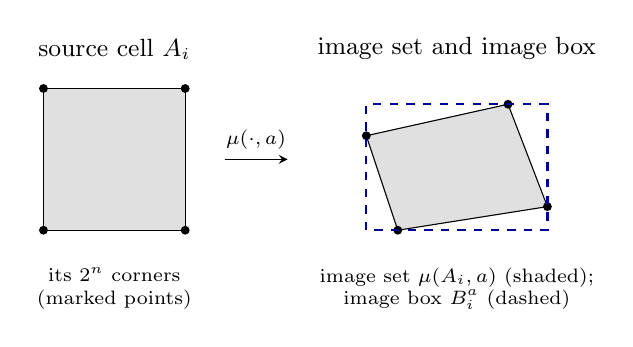
\begin{tikzpicture}[>=stealth, font=\small]
			\node[anchor=south] at (1.3,2.75) {source cell $A_i$};
			\fill[black!12] (0.4,0.7) rectangle (2.2,2.5);
			\draw (0.4,0.7) rectangle (2.2,2.5);
			\foreach \x/\y in {0.4/0.7, 2.2/0.7, 0.4/2.5, 2.2/2.5}
			\fill (\x,\y) circle (1.6pt);
			\node[anchor=north, font=\scriptsize, align=center] at (1.3,0.35)
			{its $2^n$ corners\\ (marked points)};
			\draw[->] (2.7,1.6) -- (3.5,1.6)
			node[midway, above, font=\scriptsize] {$\mu(\cdot, a)$};
			\begin{scope}[shift={(3.9,0)}]
				\node[anchor=south] at (1.75,2.75) {image set and image box};
				\fill[black!12] (0.6,1.9) -- (2.4,2.3) -- (2.9,1.0) -- (1.0,0.7) -- cycle;
				\draw (0.6,1.9) -- (2.4,2.3) -- (2.9,1.0) -- (1.0,0.7) -- cycle;
				\foreach \x/\y in {0.6/1.9, 2.4/2.3, 2.9/1.0, 1.0/0.7}
				\fill (\x,\y) circle (1.6pt);
				\draw[blue!60!black, thick, dashed] (0.6,0.7) rectangle (2.9,2.3);
				\node[anchor=north, font=\scriptsize, align=center] at (1.75,0.35)
				{image set $\mu(A_i, a)$ (shaded);\\ image box $B_i^a$ (dashed)};
			\end{scope}
		\end{tikzpicture}
		
		\caption{The image box. Left: the source cell, drawn as in
			Figure~\ref{fig:cellstate}, with its $2^n$ corners marked as in
			Figure~\ref{fig:corners}. Right: the mean map sends the cell to its
			image set~\eqref{eq:imageset}; the marked points are the images of
			the corners. By \hyperref[ass:sysclass]{Assumption~(iii)} the
			smallest and largest value of each coordinate over the image is
			attained at a corner image, so the dashed box they span, the image
			box~\eqref{eq:imageboxdef}, encloses the whole image set.}
		\label{fig:imagebox}
	\end{figure}
	
	The image box is an intermediate object: it determines the transitions of one source cell under one action and is then discarded, and it is never itself a state of the IMDP. It typically intersects several of the fixed target cells of Section~\ref{sec:abs:partition} (Figure~\ref{fig:targetcells}), and each target cell the box intersects becomes one transition of the source cell, carrying its own probability interval computed against the box; the cells themselves remain disjoint, it is the box that spans several of them. Because the box is an interval in every dimension, the intersected grid cells form a contiguous, axis-aligned block in index space: a source cell transitions into a block of target cells, possibly together with the terminal representative and the safe sink, and into no grid target outside the block.
	
	\begin{figure}[h]
		\centering
		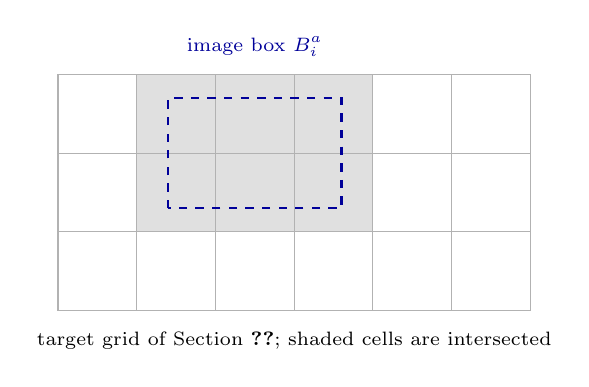
\begin{tikzpicture}[>=stealth, font=\small]
			\fill[black!12] (1,1) rectangle (4,3);
			\draw[gray!60, thin, step=1] (0,0) grid (6,3);
			\draw[blue!60!black, thick, dashed] (1.4,1.3) rectangle (3.6,2.7);
			\node[anchor=south, font=\scriptsize, blue!60!black] at (2.5,3.1)
			{image box $B_i^a$};
			\node[anchor=north, font=\scriptsize] at (3,-0.15)
			{target grid of Section~\ref{sec:abs:partition};
				shaded cells are intersected};
		\end{tikzpicture}
		\caption{The image box laid over the target grid. The grid is the
			fixed partition of Figure~\ref{fig:cellstate}; the dashed box is the
			image box of Figure~\ref{fig:imagebox}, in general not aligned to the
			grid. Each of the six shaded cells it intersects becomes one
			transition of the source cell; the box is discarded once the
			transitions are recorded.}
		\label{fig:targetcells}
	\end{figure}
	
	A single box encloses the image because the image set is connected: by \hyperref[ass:sysclass]{Assumption~(ii)} the mean map is continuous for each fixed action, and a continuous map sends the connected source cell to a connected image set. Continuity is required of the dynamics under each fixed action only. The action-selection logic of a controller is typically discontinuous across the state space, and that discontinuity never enters an image-box computation: it is confined to the separate controller component, which only decides which action's transitions apply to each cell (Section~\ref{sec:abs:full}). Generically, if the concrete system has hybrid dynamics, then a hybrid jump could split the image into disjoint pieces, and the construction would then need a union of image boxes per cell; computing per action is what removes that case here.
	
	\paragraph{Per-dimension factor intervals.}
	The factorisation~\eqref{eq:kernelfactor} of
	\hyperref[ass:sysclass]{Assumption~(i)}, instantiated at the target
	cell, reads
	\begin{equation}
		T_x(A_j \mid s, a) \;=\; \prod_{d=1}^{n} T_{x,d}\bigl(\, [\ell^j_d, h^j_d) \,\big|\, s, a \,\bigr),
		\label{eq:factorise}
	\end{equation}
	where
	\begin{itemize}
		\item $[\ell^j_d, h^j_d)$ is the target cell's interval in dimension
		$d$, as in~\eqref{eq:cellbox}, so that $A_j = \prod_d [\ell^j_d, h^j_d)$;
		\item $T_{x,d}$ is the one-dimensional factor of~\eqref{eq:kernelfactor}.
	\end{itemize}
	Each factor on the right of~\eqref{eq:factorise} is bracketed by an
	interval valid for every $s \in A_i$, and the transition interval is
	the product of the factor brackets, Equation~\eqref{eq:product}. The
	two kinds of dimension give two kinds of factor bracket.
	
	In a \emph{deterministic} dimension ($\sigma_d = 0$) the factor is
	the indicator of the event $\mu_d(s, a) \in [\ell^j_d, h^j_d)$: it
	equals $1$ for a continuous state whose mean lands inside the target
	interval and $0$ otherwise. Over the source cell, the mean
	$\mu_d(s, a)$ ranges exactly over the image interval
	$[\mu_d^{\text{lo}}, \mu_d^{\text{hi}}]$, so the tightest bracket
	valid for every continuous state of the cell is
	\begin{equation}
		\bigl[\,f_{\text{lo}},\; 1\,\bigr], \qquad
		f_{\text{lo}} =
		\begin{cases}
			1 & \text{if } \mu_d^{\text{lo}} \ge \ell^j_d \text{ and }
			\mu_d^{\text{hi}} < h^j_d,\\
			0 & \text{otherwise,}
		\end{cases}
		\label{eq:flo}
	\end{equation}
	where
	\begin{itemize}
		\item $f_{\text{lo}}$ is the lower bound of the factor bracket; the
		upper bound is $1$ for every enumerated target;
		\item the first case holds when the image interval lies wholly inside
		the half-open target interval, the second when it touches or crosses
		one of its boundaries.
	\end{itemize}
	
	A factor of $[1,1]$ records a target \emph{certainly} reached in that
	dimension: the image lies at or above the lower boundary and strictly
	below the upper one, so the mean of every continuous state lands in
	the half-open target interval. A factor of $[0,1]$ records a target
	only \emph{possibly} reached, and arises in two geometries. If the
	image \emph{crosses} a boundary of the target interval, some
	continuous states of the source cell reach the target and others do
	not, and $[0,1]$ is the exact range of the indicator over the cell.
	If the image only \emph{touches} the upper boundary $h^j_d$, the
	factor $[0,1]$ is sound but may be conservative, for the reason given
	next. Only cells the image interval crosses or touches are
	enumerated, and each receives the upper bound $1$. The upper
	inequality in~\eqref{eq:flo} is strict because the cells are
	half-open (Section~\ref{sec:abs:partition}): a mean landing exactly
	on $h^j_d$ belongs to the cell above, not to the target. Touching
	images arise routinely, not only through rounding: whenever a
	dimension moves by a fixed amount $\delta_d$ equal to the cell width
	$r_d$, a source cell aligned with the grid maps exactly onto its
	neighbouring cell, and the upper endpoint of the image lands
	precisely on the shared boundary (Figure~\ref{fig:touchingimage}). A
	non-strict test would record such a touching image as certain, with
	lower bound $1$; yet a continuous state whose mean sits exactly on
	$h^j_d$ reaches the target with probability $0$, so the recorded
	lower bound would exceed the true probability and
	violate~\eqref{eq:cellcontain}. The strict test records $[0,1]$
	instead, which is sound in every case and conservative only when no
	state of the half-open source cell attains the boundary.
	
	\begin{figure}[h]
		\centering
		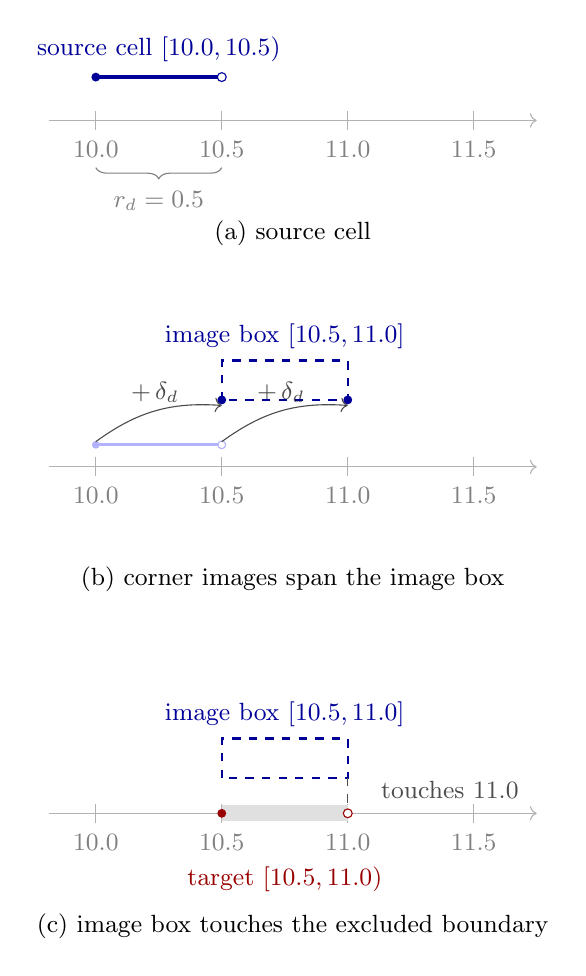
\begin{tikzpicture}[font=\small]
			% common x positions: 10.0 -> 0.6, 10.5 -> 2.2, 11.0 -> 3.8, 11.5 -> 5.4
			% ---------- Panel (a): source cell ----------
			\begin{scope}
				\draw[gray!60,->] (0.0,0) -- (6.2,0);
				\foreach \x/\lab in {0.6/{$10.0$}, 2.2/{$10.5$}, 3.8/{$11.0$}, 5.4/{$11.5$}}
				{
					\draw[gray!60] (\x,-0.12) -- (\x,0.12);
					\node[below, gray] at (\x,-0.14) {\lab};
				}
				\draw[blue!60!black, very thick] (0.6,0.55) -- (2.2,0.55);
				\fill[blue!60!black] (0.6,0.55) circle (1.6pt);
				\draw[blue!60!black, fill=white] (2.2,0.55) circle (1.6pt);
				\node[above, blue!60!black] at (1.4,0.62)
				{source cell $[10.0, 10.5)$};
				\draw[decorate, decoration={brace, mirror, amplitude=4pt}, gray]
				(0.6,-0.6) -- (2.2,-0.6)
				node[midway, below=5pt, gray] {$r_d = 0.5$};
				\node[below] at (3.1,-1.15) {(a) source cell};
			\end{scope}
			% ---------- Panel (b): corner evaluation ----------
			\begin{scope}[shift={(0,-4.4)}]
				\draw[gray!60,->] (0.0,0) -- (6.2,0);
				\foreach \x/\lab in {0.6/{$10.0$}, 2.2/{$10.5$}, 3.8/{$11.0$}, 5.4/{$11.5$}}
				{
					\draw[gray!60] (\x,-0.12) -- (\x,0.12);
					\node[below, gray] at (\x,-0.14) {\lab};
				}
				% source cell, faded, on the axis level
				\draw[blue!30, very thick] (0.6,0.28) -- (2.2,0.28);
				\fill[blue!30] (0.6,0.28) circle (1.4pt);
				\draw[blue!30, fill=white] (2.2,0.28) circle (1.4pt);
				% corner-to-corner-image arrows, kept shallow
				\draw[->, black!70] (0.6,0.32) to[bend left=20] (2.2,0.78);
				\draw[->, black!70] (2.2,0.32) to[bend left=20] (3.8,0.78);
				\node[black!70] at (1.35,0.95) {$+\,\delta_d$};
				\node[black!70] at (2.95,0.95) {$+\,\delta_d$};
				% corner images
				\fill[blue!60!black] (2.2,0.85) circle (1.6pt);
				\fill[blue!60!black] (3.8,0.85) circle (1.6pt);
				% image box drawn as a box spanning the corner images
				\draw[blue!60!black, dashed, thick]
				(2.2,0.85) rectangle (3.8,1.35);
				\node[above, blue!60!black] at (3.0,1.38)
				{image box $[10.5, 11.0]$};
				\node[below] at (3.1,-1.15)
				{(b) corner images span the image box};
			\end{scope}
			% ---------- Panel (c): image box against the target ----------
			\begin{scope}[shift={(0,-8.8)}]
				\draw[gray!60,->] (0.0,0) -- (6.2,0);
				\foreach \x/\lab in {0.6/{$10.0$}, 2.2/{$10.5$}, 3.8/{$11.0$}, 5.4/{$11.5$}}
				{
					\draw[gray!60] (\x,-0.12) -- (\x,0.12);
					\node[below, gray] at (\x,-0.14) {\lab};
				}
				% target cell as grey band with half-open endpoints
				\fill[black!12] (2.2,-0.1) rectangle (3.8,0.1);
				\fill[red!60!black] (2.2,0) circle (1.6pt);
				\draw[red!60!black, fill=white] (3.8,0) circle (1.6pt);
				\node[below, red!60!black] at (3.0,-0.55)
				{target $[10.5, 11.0)$};
				% image box above the target
				\draw[blue!60!black, dashed, thick]
				(2.2,0.45) rectangle (3.8,0.95);
				\node[above, blue!60!black] at (3.0,0.98)
				{image box $[10.5, 11.0]$};
				% touching annotation
				\draw[dashed, black!70] (3.8,0.45) -- (3.8,0.12);
				\node[right, black!70] at (4.1,0.3) {touches $11.0$};
				\node[below] at (3.1,-1.15)
				{(c) image box touches the excluded boundary};
			\end{scope}
		\end{tikzpicture}
		\caption{A touching image from an aligned step. The step
			$\delta_d = r_d = 0.5$ sends both corners of the source cell onto
			grid lines, so the image box touches the excluded upper boundary of
			the target and the factor is $[0,1]$.}
		\label{fig:touchingimage}
	\end{figure}
	
	
	In a \emph{stochastic} dimension ($\sigma_d > 0$) each step splits
	into a prediction and a landing. The mean map sends the continuous
	state to a single predicted next value, exactly as in a deterministic
	dimension. The landing is then a random draw from a Gaussian density
	centred on the prediction, with standard deviation $\sigma_d$
	(Figure~\ref{fig:predlanding}). The prediction is a function of the
	state alone; the spread around it is the noise. Three terms are kept
	distinct throughout: the \emph{prediction}, where a density is
	centred; the \emph{target window}, the half-open interval
	$[\ell^j_d, h^j_d)$ of a candidate cell; and the \emph{cell middle},
	the midpoint of that window. The factor for a target is the landing
	chance,
	\begin{equation}
		g(\mu) \;=\; \Phi\!\Bigl(\tfrac{h^j_d - \mu}{\sigma_d}\Bigr)
		- \Phi\!\Bigl(\tfrac{\ell^j_d - \mu}{\sigma_d}\Bigr),
		\label{eq:g}
	\end{equation}
	where
	\begin{itemize}
		\item $g(\mu)$ is the chance that the landing falls in the target
		window $[\ell^j_d, h^j_d)$ when the prediction is $\mu$;
		\item $\mu$ is the prediction, the value the mean map assigns to the
		continuous state;
		\item $\sigma_d$ is the noise level of the dimension, the standard
		deviation of the Gaussian, constant over the state space;
		\item $\Phi$ is the standard normal cumulative distribution function:
		$\Phi(x)$ is the chance that a standard Gaussian draw falls below
		$x$, a tabulated function available in every numerical library.
	\end{itemize}
	
	\begin{figure}[h]
		\centering
		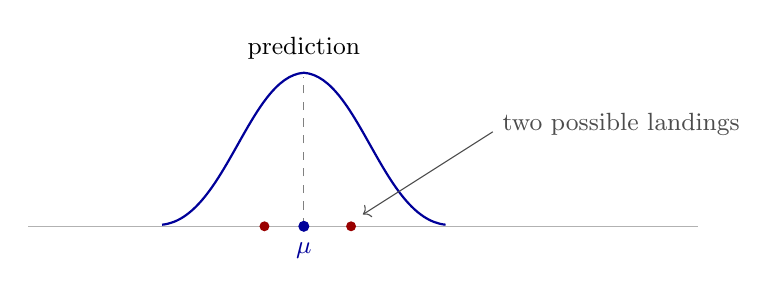
\begin{tikzpicture}[font=\small]
			\draw[gray!60] (0.5,0) -- (9.0,0);
			\draw[blue!60!black, thick]
			(2.2,0.02) .. controls (3.0,0.1) and (3.3,1.9) .. (4.0,1.95)
			.. controls (4.7,1.9) and (5.0,0.1) .. (5.8,0.02);
			\draw[dashed, gray] (4.0,0) -- (4.0,1.9);
			\fill[blue!60!black] (4.0,0) circle (2pt);
			\node[below, blue!60!black] at (4.0,-0.08) {$\mu$};
			\node[above] at (4.0,2.0) {prediction};
			\fill[red!60!black] (4.6,0) circle (1.8pt);
			\fill[red!60!black] (3.5,0) circle (1.8pt);
			\draw[->, black!70] (6.4,1.2) -- (4.75,0.15);
			\node[right, black!70, align=left] at (6.4,1.3)
			{two possible landings};
		\end{tikzpicture}
		\caption{Prediction and landing. The mean map fixes the prediction
			$\mu$; the density is fixed to it; a landing is a draw from the
			density. The construction never draws landings: it evaluates their
			chances in closed form through~\eqref{eq:g}.}
		\label{fig:predlanding}
	\end{figure}
	A source cell contains a continuum of continuous states, and each
	state has its own prediction, so the cell owns a family of identical
	densities whose positions differ. The corner
	evaluation~\eqref{eq:imagebox}, the same one used for the
	deterministic dimensions, returns the smallest and largest
	prediction, and by the monotone continuity of the mean map every
	value between them is the prediction of some state in the cell. The
	attainable predictions therefore fill the image interval
	$[\mu_d^{\text{lo}}, \mu_d^{\text{hi}}]$ exactly, and no prediction
	outside it is attainable (Figure~\ref{fig:predrange}).
	
	\begin{figure}[h]
		\centering
		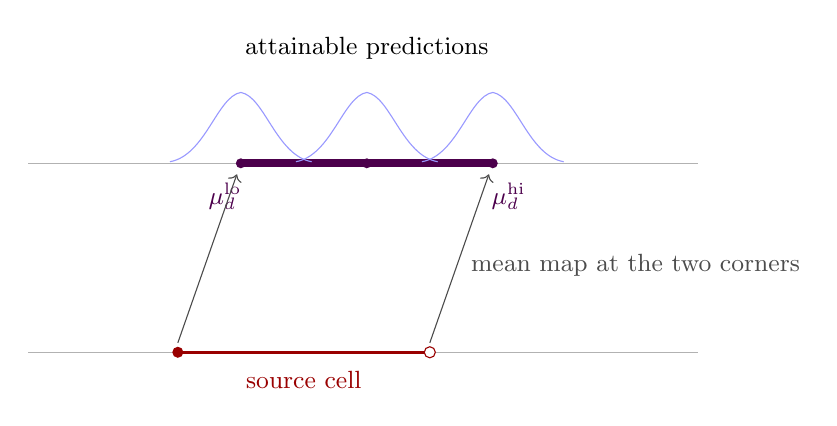
\begin{tikzpicture}[font=\small]
			\draw[gray!60] (0.5,2.4) -- (9.0,2.4);
			\draw[violet!60!black, line width=3pt] (3.2,2.4) -- (6.4,2.4);
			\node[above] at (4.8,3.6) {attainable predictions};
			\node[below, violet!60!black] at (3.0,2.28) {$\mu_d^{\text{lo}}$};
			\node[below, violet!60!black] at (6.6,2.28) {$\mu_d^{\text{hi}}$};
			\foreach \c in {3.2, 4.8, 6.4}{
				\draw[blue!40]
				(\c-0.9,2.42) .. controls (\c-0.45,2.5) and (\c-0.3,3.25) .. (\c,3.3)
				.. controls (\c+0.3,3.25) and (\c+0.45,2.5) .. (\c+0.9,2.42);
				\fill[violet!60!black] (\c,2.4) circle (1.8pt);
			}
			\draw[gray!60] (0.5,0) -- (9.0,0);
			\draw[red!60!black, very thick] (2.4,0) -- (5.6,0);
			\fill[red!60!black] (2.4,0) circle (2pt);
			\draw[red!60!black, fill=white] (5.6,0) circle (2pt);
			\node[below, red!60!black] at (4.0,-0.12) {source cell};
			\draw[->, black!70] (2.4,0.12) -- (3.15,2.26);
			\draw[->, black!70] (5.6,0.12) -- (6.35,2.26);
			\node[right, black!70] at (6.0,1.1) {mean map at the two corners};
		\end{tikzpicture}
		\caption{The attainable predictions. The mean map at the two corners
			of the source cell bounds the predictions; every value between is
			attained by some state of the cell, and none outside is. Each
			prediction on the interval carries its own density; three are drawn.}
		\label{fig:predrange}
	\end{figure}
	
	The abstraction must attach one factor to the whole cell, valid for every state in it. Different states have different predictions, hence
	different landing chances, so the factor is the range of the landing
	chance over the attainable predictions: from the smallest chance
	attained by any state of the cell to the largest. Both extremes are
	located in closed form, because the landing chance depends on the
	prediction in a simple way: it is largest when the prediction equals
	the cell middle,
	\begin{equation}
		\mu^\star \;=\; \frac{\ell^j_d + h^j_d}{2},
		\label{eq:peak}
	\end{equation}
	and it decreases as the prediction moves away from the cell middle in
	either direction, since the density is symmetric and places less mass
	on the window the further its centre lies from it. The extremes over
	the image interval follow immediately. The smallest chance is at the
	end of the interval farther from the cell middle,
	\begin{equation}
		m \;=\; \min\bigl\{g(\mu_d^{\text{lo}}),\; g(\mu_d^{\text{hi}})\bigr\},
		\label{eq:mlo}
	\end{equation}
	and the largest is at the attainable prediction closest to the cell
	middle,
	\begin{equation}
		M \;=\; g(\bar\mu),
		\label{eq:Mhi}
	\end{equation}
	where
	\begin{itemize}
		\item $\bar\mu$ is the attainable prediction closest to the cell
		middle: $\mu^\star$ itself if the image interval contains it, the
		nearer end of the interval otherwise.
	\end{itemize}
	
	
	The range $[m, M]$ is the per-transition bound
	of~\cite[Eq.~3.11]{Soudjani2013}. Both cases of $\bar\mu$ arise for a
	single source cell, because neighbouring targets have different
	middles. Figure~\ref{fig:targets} places two candidate targets
	against one image interval: the middle of the first lies inside the
	interval, the middle of the second outside.
	Figure~\ref{fig:gaussmass} then computes the bracket for each target
	in turn.
	
	\begin{figure}[h]
		\centering
		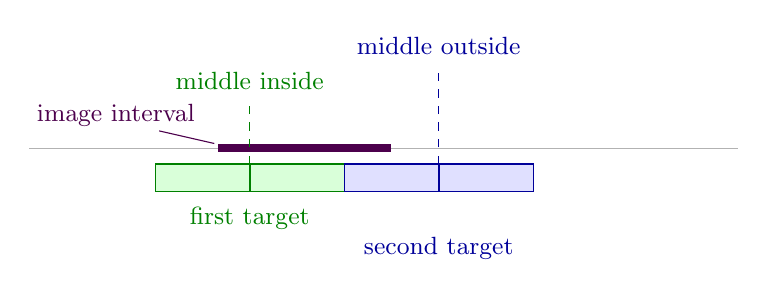
\begin{tikzpicture}[font=\small]
			\draw[gray!60] (0.2,0) -- (9.2,0);
			\draw[violet!60!black, line width=3pt] (2.6,0) -- (4.8,0);
			\node[above, violet!60!black] at (1.3,0.15) {image interval};
			\draw[violet!60!black] (1.85,0.22) -- (2.55,0.06);
			\fill[green!15] (1.8,-0.55) rectangle (4.2,-0.2);
			\draw[green!50!black] (1.8,-0.55) rectangle (4.2,-0.2);
			\draw[green!50!black, thick] (3.0,-0.55) -- (3.0,-0.2);
			\fill[blue!12] (4.2,-0.55) rectangle (6.6,-0.2);
			\draw[blue!60!black] (4.2,-0.55) rectangle (6.6,-0.2);
			\draw[blue!60!black, thick] (5.4,-0.55) -- (5.4,-0.2);
			\draw[dashed, green!50!black] (3.0,-0.2) -- (3.0,0.6);
			\node[above, green!50!black] at (3.0,0.62) {middle inside};
			\draw[dashed, blue!60!black] (5.4,-0.2) -- (5.4,1.05);
			\node[above, blue!60!black] at (5.4,1.07) {middle outside};
			\node[below, green!50!black] at (3.0,-0.63) {first target};
			\node[below, blue!60!black] at (5.4,-1.0) {second target};
		\end{tikzpicture}
		\caption{Two candidate targets against one image interval: the first
			target (green) and the second (blue), each with its middle marked.
			The first target's middle lies inside the interval; the second's lies
			outside it. The two targets are carried through
			Figure~\ref{fig:gaussmass}.}
		\label{fig:targets}
	\end{figure}
	
	\begin{figure}[h]
		\centering
		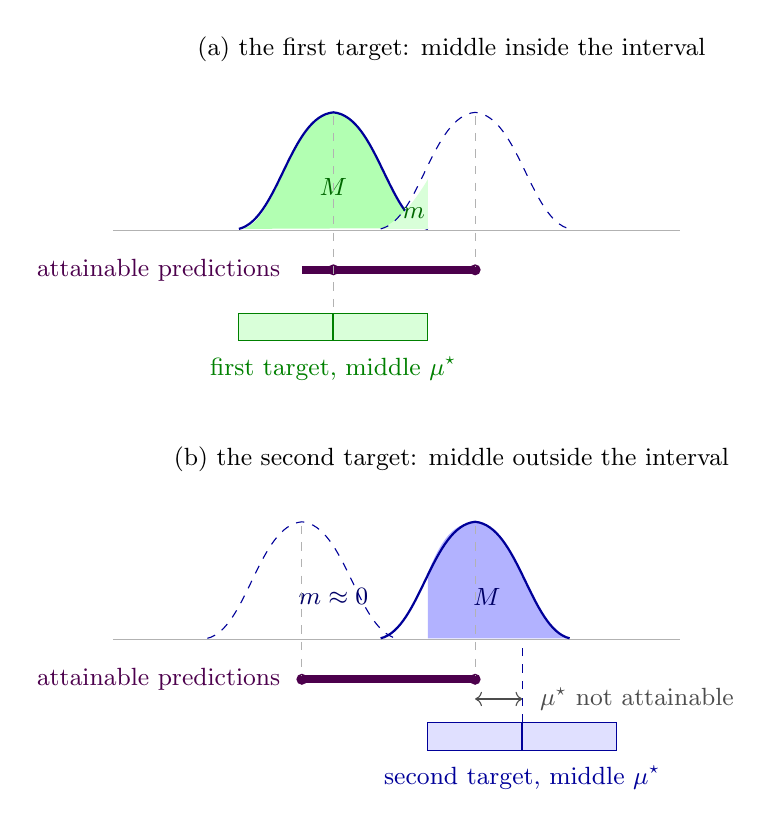
\begin{tikzpicture}[font=\small]
			\begin{scope}
				\node at (4.5,2.3) {(a) the first target: middle inside the interval};
				\draw[gray!60] (0.2,0) -- (7.4,0);
				\fill[green!30]
				(1.85,0.02) .. controls (2.3,0.14) and (2.45,1.45) .. (3.0,1.5)
				.. controls (3.55,1.45) and (3.7,0.14) .. (4.15,0.03) -- cycle;
				\draw[blue!60!black, thick]
				(1.8,0.02) .. controls (2.3,0.14) and (2.45,1.45) .. (3.0,1.5)
				.. controls (3.55,1.45) and (3.7,0.14) .. (4.2,0.02);
				\fill[green!15]
				(3.6,0.02) .. controls (3.85,0.12) and (4.05,0.4) .. (4.2,0.65)
				-- (4.2,0.02) -- cycle;
				\draw[blue!60!black, dashed]
				(3.6,0.02) .. controls (4.1,0.14) and (4.25,1.45) .. (4.8,1.5)
				.. controls (5.35,1.45) and (5.5,0.14) .. (6.0,0.02);
				\node[green!40!black] at (3.0,0.55) {$M$};
				\node[green!40!black] at (4.02,0.22) {$m$};
				\draw[violet!60!black, line width=3pt] (2.6,-0.5) -- (4.8,-0.5);
				\node[left, violet!60!black] at (2.45,-0.5) {attainable predictions};
				\fill[violet!60!black] (3.0,-0.5) circle (2pt);
				\fill[violet!60!black] (4.8,-0.5) circle (2pt);
				\draw[dashed, gray!60] (3.0,1.45) -- (3.0,-1.05);
				\draw[dashed, gray!60] (4.8,1.45) -- (4.8,-0.46);
				\fill[green!15] (1.8,-1.4) rectangle (4.2,-1.05);
				\draw[green!50!black] (1.8,-1.4) rectangle (4.2,-1.05);
				\draw[green!50!black, thick] (3.0,-1.4) -- (3.0,-1.05);
				\node[below, green!50!black] at (3.0,-1.48) {first target, middle $\mu^\star$};
			\end{scope}
			\begin{scope}[shift={(0,-5.2)}]
				\node at (4.5,2.3) {(b) the second target: middle outside the interval};
				\draw[gray!60] (0.2,0) -- (7.4,0);
				\fill[blue!30]
				(4.2,0.02) -- (4.2,0.85)
				.. controls (4.4,1.35) and (4.55,1.47) .. (4.8,1.5)
				.. controls (5.35,1.45) and (5.5,0.14) .. (6.0,0.02) -- cycle;
				\draw[blue!60!black, thick]
				(3.6,0.02) .. controls (4.1,0.14) and (4.25,1.45) .. (4.8,1.5)
				.. controls (5.35,1.45) and (5.5,0.14) .. (6.0,0.02);
				\draw[blue!60!black, dashed]
				(1.4,0.02) .. controls (1.9,0.14) and (2.05,1.45) .. (2.6,1.5)
				.. controls (3.15,1.45) and (3.3,0.14) .. (3.8,0.02);
				\node[blue!40!black] at (4.95,0.55) {$M$};
				\node[blue!40!black] at (3.0,0.55) {$m \approx 0$};
				\draw[violet!60!black, line width=3pt] (2.6,-0.5) -- (4.8,-0.5);
				\node[left, violet!60!black] at (2.45,-0.5) {attainable predictions};
				\fill[violet!60!black] (4.8,-0.5) circle (2pt);
				\fill[violet!60!black] (2.6,-0.5) circle (2pt);
				\draw[dashed, gray!60] (4.8,1.45) -- (4.8,-0.46);
				\draw[dashed, gray!60] (2.6,1.45) -- (2.6,-0.46);
				\draw[<->, black!70] (4.8,-0.75) -- (5.4,-0.75);
				\node[right, black!70] at (5.5,-0.75) {$\mu^\star$ not attainable};
				\draw[dashed, blue!60!black] (5.4,-1.05) -- (5.4,0);
				\fill[blue!12] (4.2,-1.4) rectangle (6.6,-1.05);
				\draw[blue!60!black] (4.2,-1.4) rectangle (6.6,-1.05);
				\draw[blue!60!black, thick] (5.4,-1.4) -- (5.4,-1.05);
				\node[below, blue!60!black] at (5.4,-1.48) {second target, middle $\mu^\star$};
			\end{scope}
		\end{tikzpicture}
		\caption{The bracket computed for each target of
			Figure~\ref{fig:targets}, over the same image interval. Each density
			stands on its placement, marked by a violet dot on the interval of
			attainable predictions and tied to the peak by a dashed guide; the
			shaded area over the target, in the target's colour, is the landing
			chance. (a) The first target's middle is attainable, so the solid
			density is placed there, $\bar\mu = \mu^\star$, giving the largest
			chance $M$~\eqref{eq:Mhi}; the dashed density at the far end gives
			the smallest, $m$~\eqref{eq:mlo}. (b) The second target's middle is
			not attainable: the solid density is placed at the interval's end,
			the closest allowed position, and the far-end density does not reach
			the target, so $m$ is negligible.}
		\label{fig:gaussmass}
	\end{figure}
	
	Each candidate target is bracketed independently, over the same image
	interval; repeating the computation per target gives one bracket per
	transition. The brackets are bounds, not shares of a fixed total: a
	target whose window lies away from the image interval receives a
	bracket small at both ends, with the mass appearing in the
	transitions to the cells the image covers. 
	
	The candidate targets are the cells beneath the image interval
	extended on each side by the noise reach
	$n_{\mathrm{cut}}\,\sigma_d$, where $n_{\mathrm{cut}}$ is a cutoff
	parameter. Cells beyond the window are assigned probability zero, an
	approximation of at most $\Phi(-n_{\mathrm{cut}})$ beyond each end of
	the window, per transition; $n_{\mathrm{cut}}$ is chosen large enough
	that this mass lies below the numerical tolerance of the containment
	certificate and the precision of the model checker. The experiments
	use $n_{\mathrm{cut}} = 6$, for which the ignored mass is of order
	$10^{-9}$ (Section~\ref{sec:cs:exp}).
	
	\paragraph{State-independence of the noise.}
	The bracket~\eqref{eq:mlo}--\eqref{eq:Mhi} evaluates $g$ at a single
	noise magnitude $\sigma_d$ per source cell. It is therefore valid
	only under the state-independence of the noise required by
	\hyperref[ass:sysclass]{Assumption~(i)}: were $\sigma_d$ to vary with
	the state, $g$ would have to be ranged over the spread of $\sigma_d$
	across the cell as well as over the image.
	Algorithm~\ref{alg:imagebox} checks this part of the assumption at
	construction time: it records the noise at every corner of the source
	cell, requires the values to agree to numerical tolerance, and aborts
	otherwise.

	
	\paragraph{Truncation of the stochastic tail.}
	The grid covers a bounded interval $[b_{\min}, b_{\max}]$ of the
	stochastic dimension, its \emph{grid band}. The cells of the
	dimension partition the band: $b_{\min}$ is the lower edge of the
	first cell and $b_{\max}$ the upper edge of the last. A density whose
	prediction lies near an end of the band places part of its mass past
	that end, outside the grid (Figure~\ref{fig:truncation}). The
	abstraction assumes that the dimension remains inside the band, so
	this mass must be removed from the factors. Each factor is divided by
	the probability that the landing lies inside the band. Away from the
	ends of the band this probability is $1$ and the factor is unchanged;
	near an end it is smaller than $1$, and the division raises the
	factor to compensate for the removed mass.
	
	\begin{figure}[h]
		\centering
		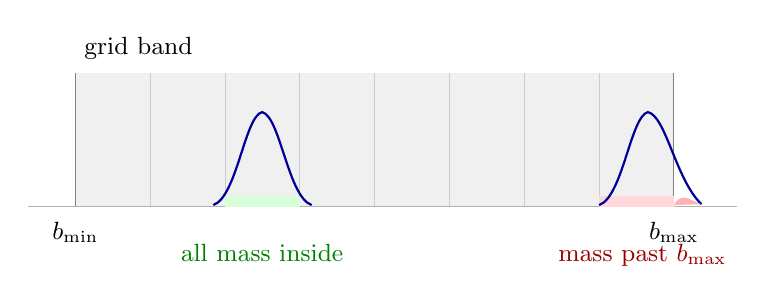
\begin{tikzpicture}[font=\small]
			\fill[black!6] (0.8,0) rectangle (8.4,1.7);
			\draw[gray] (0.8,0) -- (0.8,1.7);
			\draw[gray] (8.4,0) -- (8.4,1.7);
			\foreach \x in {1.75, 2.7, 3.65, 4.6, 5.55, 6.5, 7.45}
			\draw[gray!40] (\x,0) -- (\x,1.7);
			\node[below] at (0.8,-0.08) {$b_{\min}$};
			\node[below] at (8.4,-0.08) {$b_{\max}$};
			\node[above] at (1.6,1.75) {grid band};
			\draw[gray!60] (0.2,0) -- (9.2,0);
			\fill[green!15] (2.7,0) rectangle (3.65,0.14);
			\draw[blue!60!black, thick]
			(2.55,0.02) .. controls (2.85,0.12) and (2.95,1.15) .. (3.17,1.2)
			.. controls (3.4,1.15) and (3.5,0.12) .. (3.8,0.02);
			\node[below, green!50!black] at (3.17,-0.35) {all mass inside};
			\fill[red!15] (7.45,0) rectangle (8.4,0.14);
			\draw[blue!60!black, thick]
			(7.45,0.02) .. controls (7.75,0.12) and (7.85,1.15) .. (8.07,1.2)
			.. controls (8.3,1.15) and (8.42,0.35) .. (8.75,0.03);
			\fill[red!30]
			(8.4,0.02) .. controls (8.5,0.2) and (8.6,0.08) .. (8.75,0.03)
			-- (8.4,0.02) -- cycle;
			\node[below, red!60!black] at (8.0,-0.35) {mass past $b_{\max}$};
		\end{tikzpicture}
		\caption{Truncation of the stochastic tail. The cells of the
			stochastic dimension partition the grid band $[b_{\min}, b_{\max}]$.
			For an interior cell all mass lands inside the band and the division
			changes nothing; for a cell at an end of the band, part of the mass
			falls past the edge and the division compensates for its removal.}
		\label{fig:truncation}
	\end{figure}
	
	The divisor is the probability that the landing lies inside the band,
	\begin{equation}
		\Pi(\mu) = \Phi\!\Bigl(\tfrac{b_{\max}-\mu}{\sigma_d}\Bigr)
		- \Phi\!\Bigl(\tfrac{b_{\min}-\mu}{\sigma_d}\Bigr),
		\label{eq:inband}
	\end{equation}
	where
	\begin{itemize}
		\item $\Pi(\mu)$ is the probability that a landing with prediction
		$\mu$ lies inside the band $[b_{\min}, b_{\max}]$.
	\end{itemize}
	
	
	For a single continuous state, the stored probability of a target
	cell is the conditional probability of reaching it given that the
	landing lies inside the band. This conditional probability is the
	quotient of the landing chance by the divisor,
	\begin{equation}
		\frac{g(\mu)}{\Pi(\mu)},
		\label{eq:quotient}
	\end{equation}
	where
	\begin{itemize}
		\item $g(\mu)$ and $\Pi(\mu)$ are evaluated at the prediction $\mu$
		of that state.
	\end{itemize}
	Every value in the image interval is the prediction of some state of
	the source cell, and each such value has its own divisor. The stored
	factor must therefore bracket the quotient over the whole image
	interval. The divisor is largest for a prediction at the midpoint of the band
	and shrinks toward the band's ends. Over the image interval, the
	largest divisor is therefore found at the point of the interval
	closest to the band midpoint, and the smallest at the end of the
	interval farthest from it. The lower end of the stored factor is
	divided by the largest divisor and the upper end by the smallest, so
	that the lower end can only decrease and the upper end only increase:
	\begin{equation}
		\bigl[\,m/\Pi_{\text{hi}},\; M/\Pi_{\text{lo}}\,\bigr],
		\label{eq:trunc}
	\end{equation}
	where
	\begin{itemize}
		\item $\Pi_{\text{lo}}$ and $\Pi_{\text{hi}}$ are the smallest and
		largest values of the divisor over the image interval.
	\end{itemize}
	
	The stored ends are safe for every state of the cell. Each state's
	conditional probability is built from a landing chance no smaller
	than $m$ and no larger than $M$, and a divisor no smaller than
	$\Pi_{\text{lo}}$ and no larger than $\Pi_{\text{hi}}$, so it cannot
	fall below the stored lower end nor exceed the stored upper end:
	\begin{equation}
		\frac{m}{\Pi_{\text{hi}}} \;\le\; \frac{g(\mu)}{\Pi(\mu)} \;\le\;
		\frac{M}{\Pi_{\text{lo}}}
		\qquad \forall \mu \in [\mu_d^{\text{lo}}, \mu_d^{\text{hi}}],
		\label{eq:truncsound}
	\end{equation}
	where
	\begin{itemize}
		\item $g(\mu)$ and $\Pi(\mu)$ are the landing chance~\eqref{eq:g}
		and the divisor~\eqref{eq:inband} at the prediction $\mu$;
		\item $m$ and $M$ are the ends of the landing-chance
		bracket~\eqref{eq:mlo}--\eqref{eq:Mhi}, and $\Pi_{\text{lo}}$ and
		$\Pi_{\text{hi}}$ the smallest and largest divisor over the image
		interval, as in~\eqref{eq:trunc};
		\item $[\mu_d^{\text{lo}}, \mu_d^{\text{hi}}]$ is the image
		interval~\eqref{eq:imagebox}.
	\end{itemize}
		
	
	The two factor types are visible in the generated model. A
	deterministic dimension has no randomness, so its factor places the
	whole outcome at one point. The ends of that factor are therefore
	$0$ or $1$, and its value can turn on which cell owns a shared
	boundary. A
	stochastic dimension spreads its outcome as a density, and a single
	point carries no mass under a density, so boundary ownership does not
	affect its factor, and the factor's ends are fractional. A
	transition's interval is the product~\eqref{eq:product} of one factor
	per dimension, and every fractional entry in the model is the
	stochastic factor showing through that product
	(Figure~\ref{fig:atomvsdensity}).
	
	\begin{figure}[h]
		\centering
		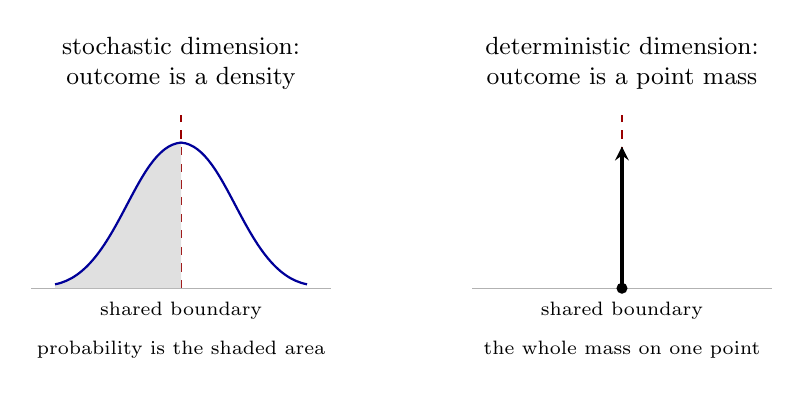
\begin{tikzpicture}[>=stealth, font=\small]
			\node[anchor=south, align=center] at (2.1,2.9)
			{stochastic dimension:\\outcome is a density};
			\draw[gray!60] (0.2,0.5) -- (4.0,0.5);
			\draw[red!60!black, thick, dashed] (2.1,0.5) -- (2.1,2.7);
			\node[below, font=\scriptsize] at (2.1,0.45) {shared boundary};
			\fill[black!12] (0.5,0.55) .. controls (1.3,0.7) and (1.5,2.3) .. (2.1,2.35)
			-- (2.1,0.5) -- (0.5,0.5) -- cycle;
			\draw[blue!60!black, thick] (0.5,0.55) .. controls (1.3,0.7) and (1.5,2.3) .. (2.1,2.35)
			.. controls (2.7,2.3) and (2.9,0.7) .. (3.7,0.55);
			\node[anchor=north, font=\scriptsize] at (2.1,-0.05)
			{probability is the shaded area};
			\begin{scope}[shift={(5.6,0)}]
				\node[anchor=south, align=center] at (2.1,2.9)
				{deterministic dimension:\\outcome is a point mass};
				\draw[gray!60] (0.2,0.5) -- (4.0,0.5);
				\draw[red!60!black, thick, dashed] (2.1,0.5) -- (2.1,2.7);
				\node[below, font=\scriptsize] at (2.1,0.45) {shared boundary};
				\draw[->, very thick] (2.1,0.5) -- (2.1,2.3);
				\fill (2.1,0.5) circle (2pt);
				\node[anchor=north, font=\scriptsize] at (2.1,-0.05)
				{the whole mass on one point};
			\end{scope}
		\end{tikzpicture}
		\caption{The two factor types. In a stochastic dimension (left) the
			outcome spreads as a density; a single point carries no mass, so
			which cell owns a shared boundary does not affect the factor. In a
			deterministic dimension (right) the outcome is a point mass, drawn
			on the boundary; which cell owns the boundary decides which cell
			receives the mass, under the half-open convention of
			Section~\ref{sec:abs:partition}.}
		\label{fig:atomvsdensity}
	\end{figure}
			

	\paragraph{Terminal routing.}
	A designated terminal region absorbs the runs that enter it. The
	routing fills the row of any source cell whose image meets the
	region, given a membership test that classifies the image as wholly
	inside, partly inside, or outside the region. When the image is
	wholly inside, no factors are computed: the row is a single
	transition to the terminal representative
	(Section~\ref{sec:abs:partition}), with interval set directly to
	$[1,1]$. When the image is partly inside, the representative is added
	as a target beside the grid targets, with interval set directly to
	$[0,1]$; the grid targets' intervals are computed by the factor
	construction as before, and no grid target is enumerated inside the
	region.
	
	The provided membership test covers a region bounded in a single
	deterministic dimension: the region lies beyond a boundary value in
	that dimension, the \emph{terminal boundary}. The dimension is
	deterministic, so the image box holds the actual next coordinate of
	every state of the source cell, and membership is read off the image
	box alone. Each state then either enters the region or does not, so
	$[0,1]$ is the exact range for a partly inside image. Grid targets in
	the bounded dimension are enumerated only up to the terminal
	boundary. Certain coverage is tested against the whole image, so a
	grid target straddling the terminal boundary receives the lower bound
	$0$. A richer region, over several dimensions or with a stochastic
	threshold, requires a richer membership test; the routing itself is
	unchanged.
	

	\paragraph{Escape in the deterministic dimensions.}
	The grid models a bounded window of each dimension, and the dynamics
	are not confined to it. Unless floored or capped at the corresponding
	state-space bound, the image in a deterministic dimension can extend
	beyond the grid at either end. A state carried past the edge leaves
	the modelled window, and the safe sink of
	Section~\ref{sec:abs:partition} is the outcome that records this.
	Whether an image point has left the grid follows from the half-open
	convention of Section~\ref{sec:abs:partition}. The grid's top edge is
	the excluded upper edge of the last cell, so a point exactly on it
	lies outside; the grid's bottom edge is the included lower edge of
	the first cell, so a point exactly on it lies inside. When the whole
	image has left the grid, no factors are computed, and the row is a
	single transition to the sink with interval set directly to $[1,1]$.
	When part of the image leaves the grid, the sink is added as a target
	beside the enumerated grid targets, with interval set directly to
	$[0,1]$, the exact range over a cell containing both escaping and
	non-escaping states. One grid edge is excepted from the sink routing.
	In the dimension that carries the terminal region, the grid ends at
	the terminal boundary, and the states beyond that edge lie inside the
	terminal region rather than outside the model. An image crossing that
	edge enters the region and is routed to the terminal representative,
	as the absorbing definition of Section~\ref{sec:abs:partition}
	prescribes. The sink routing is required for soundness in the sense
	of Section~\ref{sec:abs:sound}. Mass that leaves the grid must remain
	representable within its interval row, and a wholly escaped image
	with no sink target would produce an invalid IMDP.
	
	\paragraph{Product over dimensions.}
	The factor brackets are computed per dimension, and a transition
	needs one interval for the whole step. For the product kernel
	of~\eqref{eq:kernelfactor}, the step succeeds when every dimension
	lands in its slice of the target, so the brackets multiply, and the
	interval stored for the target cell with per-dimension indices
	$(k_1, \dots, k_n)$ is
	\begin{equation}
		p_{\min} = \prod_{d=1}^{n} f^{d}_{\text{lo}}, \qquad
		p_{\max} = \prod_{d=1}^{n} f^{d}_{\text{hi}},
		\label{eq:product}
	\end{equation}
	where
	\begin{itemize}
		\item $f^{d}_{\text{lo}}$ and $f^{d}_{\text{hi}}$ are the ends of the
		factor bracket of dimension $d$, evaluated for the target's cell
		$k_d$ in that dimension;
		\item $n$ is the number of dimensions.
	\end{itemize}
	Each index combination selects one grid cell, and the flattening of
	Section~\ref{sec:abs:partition} assigns every grid cell a single
	identifier, so distinct combinations always write to distinct
	targets. Combinations whose upper product lies below tolerance are
	discarded; the discarded mass sits below the numerical tolerance of
	the containment certificate (Section~\ref{sec:abs:sound}). A lower
	product of $0$ is stored as $0$. For a target only possibly reached,
	some states of the source cell have true probability $0$, and the
	stored interval must contain that value.\newline
	

	Three procedures carry out the row construction. The first evaluates
	the corners of a source cell and returns the image
	box~\eqref{eq:imagebox}. The second brackets the landing
	chance~\eqref{eq:g} of a single target window over the image
	interval, returning the ends~\eqref{eq:mlo}--\eqref{eq:Mhi}. The
	third calls both and assembles a full row of the IMDP, the transition
	intervals of the product~\eqref{eq:product}. \newline
	
	Algorithm~\ref{alg:imagebox} implements the corner
	evaluation~\eqref{eq:imagebox} and checks the noise
	state-independence required by
	\hyperref[ass:sysclass]{Assumption~(i)}. The strict test
	of~\eqref{eq:flo} is exact only at the delimiting edge values, so the
	corners are evaluated at the stored edges of~\eqref{eq:bins}.
	
	\begin{algorithm}[H]
		\caption{$\textsc{ImageBox}$: corner evaluation of the image box, with the noise check.}
		\label{alg:imagebox}
		\begin{algorithmic}[1]
			\Require the stored edges~\eqref{eq:bins} of the source cell; action $a$
			\Ensure image interval $[\mu^{\text{lo}}_d, \mu^{\text{hi}}_d]$ and noise $\sigma_d$ per dimension $d$
			\State evaluate the next state and the noise at every corner of the cell, every combination of the stored edges, under $a$
			\ForAll{dimensions $d$}
			\State $[\mu^{\text{lo}}_d, \mu^{\text{hi}}_d] \gets$ smallest and largest next value over the corners
			\If{the noise differs across the corners beyond tolerance} \textbf{raise} (noise not state-independent) \EndIf
			\State $\sigma_d \gets$ the common noise
			\EndFor
			\State \Return the intervals and the noise
		\end{algorithmic}
	\end{algorithm}
	

	Algorithm~\ref{alg:boxprob} returns the smallest and largest
	landing chance over the image interval, the ends
	of~\eqref{eq:mlo} and~\eqref{eq:Mhi}. It applies to the
	stochastic dimensions only.
	
	\begin{algorithm}[H]
		\caption{$\textsc{BoxProbRange}$: the range of the landing chance over the image interval.}
		\label{alg:boxprob}
		\begin{algorithmic}[1]
			\Require the image interval $[\mu_d^{\text{lo}}, \mu_d^{\text{hi}}]$ of~\eqref{eq:imagebox}; the target window $[\ell^j_d, h^j_d)$ of the candidate cell; the noise level $\sigma_d > 0$
			\Ensure $(m, M)$, the smallest and largest landing chance over the image interval
			\State evaluate the landing chance~\eqref{eq:g} at both ends of the image interval
			\State $m \gets$ the smaller of the two values, as in~\eqref{eq:mlo}
			\State $M \gets$ the landing chance at the attainable prediction closest to the cell middle, as in~\eqref{eq:Mhi}
			\State \Return $(m, M)$
		\end{algorithmic}
	\end{algorithm}


	Algorithm~\ref{alg:intervals} assembles one row of the IMDP from
	the terminal and escape routing, the factor brackets
	of~\eqref{eq:flo} and~\eqref{eq:trunc}, and the
	product~\eqref{eq:product}.
	
	\begin{algorithm}[H]
		\caption{$\textsc{RowIntervals}$: the transition intervals of one source cell under one action.}
		\label{alg:intervals}
		\begin{algorithmic}[1]
			\Require the stored edges~\eqref{eq:bins} of the source cell; action $a$; the grid and terminal region of Section~\ref{sec:abs:partition}
			\Ensure one row of the IMDP, an interval~\eqref{eq:cellcontain} per reachable target
			\State $[\mu_d^{\text{lo}}, \mu_d^{\text{hi}}]$ and $\sigma_d$, per dimension $d$ $\gets \textsc{ImageBox}$ (Algorithm~\ref{alg:imagebox})
			\If{image wholly inside the terminal region} \Return terminal representative, $[1,1]$ \EndIf
			\If{image wholly outside the grid in a deterministic dimension} \Return sink, $[1,1]$ \EndIf
			\ForAll{stochastic dimensions $d$ ($\sigma_d > 0$)}
			\State $\Pi_{\text{lo}}, \Pi_{\text{hi}} \gets$ smallest and largest divisor~\eqref{eq:inband} over $[\mu_d^{\text{lo}}, \mu_d^{\text{hi}}]$
			\State candidate targets $\gets$ cells beneath $[\mu_d^{\text{lo}}, \mu_d^{\text{hi}}]$ extended by the noise reach $n_{\mathrm{cut}}\sigma_d$
			\ForAll{candidate targets $k$}
			\State $(m, M) \gets \textsc{BoxProbRange}$ on the window of $k$ (Algorithm~\ref{alg:boxprob})
			\State $[f^d_{\text{lo}},\, f^d_{\text{hi}}]$ of $k$ $\gets$ the truncated bracket~\eqref{eq:trunc}
			\EndFor
			\EndFor
			\ForAll{deterministic dimensions $d$ ($\sigma_d = 0$)}
			\ForAll{cells $k$ the image crosses or touches, up to the terminal boundary}
			\State $[f^d_{\text{lo}},\, f^d_{\text{hi}}]$ of $k$ $\gets [f_{\text{lo}},\, 1]$ of~\eqref{eq:flo}
			\EndFor
			\EndFor
			\State row $\gets$ one transition per factor combination, interval the product~\eqref{eq:product}; drop combinations below tolerance
			\If{image partly inside the terminal region} add terminal representative, $[0,1]$ \EndIf
			\If{image partly outside the grid in a deterministic dimension, terminal edge excepted} add sink, $[0,1]$ \EndIf
			\State \Return the row
		\end{algorithmic}
	\end{algorithm}
	
	\subsection{Soundness of the abstraction}
	\label{sec:abs:sound}
	
	The IMDP stands in for the continuous system at verification time,
	and the stand-in is sound when every answer computed on it covers
	the continuous system. The preservation result
	of~\cite{DAK12} (Section~\ref{sec:bg:robust}) reduces this to one
	hypothesis on the construction: the per-transition
	containment~\eqref{eq:cellcontain}, that every stored interval
	contains the true transition probability of every continuous
	state of its source cell. This subsection establishes the
	hypothesis twice over, by the design of the construction and by a
	test that recomputes the true probabilities from the system
	itself.
	
	\paragraph{Containment by design.}
	The corner evaluation~\eqref{eq:imagebox} returns the exact range
	of the mean map over the source cell, so the image box encloses
	the image of every continuous state of the cell. The
	deterministic factor~\eqref{eq:flo} is exact with respect to the
	image box under the half-open convention, the stochastic factor
	brackets the truncated landing chance over the whole image
	interval~\eqref{eq:truncsound}, and the product~\eqref{eq:product}
	of the factor brackets encloses the factorised
	kernel~\eqref{eq:kernelfactor}. Every stored interval therefore
	satisfies~\eqref{eq:cellcontain}. Under this containment, every
	one-step law of the continuous system is a selection of the
	Markov set-chain that the IMDP denotes, and the verified bracket
	$[P_{\min}, P_{\max}]$ of Section~\ref{sec:bg:robust} covers the
	property value of the continuous system~\cite{DAK12}.
	
	\paragraph{The containment certificate.}
	The certificate compares the abstraction against the system it
	abstracts, by two independent computations. On one side stands
	the stored interval, the $[p_{\min}, p_{\max}]$
	of~\eqref{eq:cellcontain} that the construction computed from the
	corners of a source cell. On the other stands the true transition
	probability at a single continuous state: the deterministic
	coordinates advanced by the system's own dynamics
	of \hyperref[ass:sysclass]{Assumption~(i)}, evaluated at that one
	state, and the stochastic coordinates integrated as the truncated
	Gaussian of~\eqref{eq:trunc}. The true side uses no cell, no
	corner, and no interval of the construction; the two sides share
	only the definitions both must speak, the boundary convention and
	the noise truncation.
	
	A cell holds uncountably many continuous states, so the true side
	is evaluated at a finite sample of them and the design argument
	above covers the rest. The samples are evenly spaced values in
	each dimension, from the cell's lower edge to its upper edge,
	combined across dimensions: $s$ values per dimension give $s^n$
	sampled states per cell, and the certified instantiation uses
	three per dimension, twenty-seven states per cell. The placement
	respects the half-open convention of
	Section~\ref{sec:abs:partition}. The lowest value lies exactly on
	the lower edge, which the cell owns; the upper edge does not
	belong to the cell, so the highest value is the largest
	floating-point coordinate below it. At each sampled state the
	test computes the true probability of every reachable target and
	checks it against the stored interval to a fixed numerical
	tolerance, recording the excess of any violation. The check runs
	for every source cell, every action, and every reachable target
	of the grid. Four further checks run per row. A stored lower
	bound above tolerance must be met at every sampled state,
	including a state whose one-step law does not reach the target. A
	row must contain at least one transition. The row's interval ends
	must admit a probability distribution, the upper ends summing to
	at least one and the lower ends to at most one. A sampled state
	whose image in a deterministic dimension has left the grid must
	find the sink transition in the stored row. A run of the test
	over the whole grid is the certificate of one configuration.
	
	\begin{notebox}[title=Scope of the soundness claim]
		The claim covers the modelled system, not the raw physics.
		Any cross-dimension correlation the raw physics carries is
		removed in adopting the factorised
		kernel~\eqref{eq:kernelfactor}, and the removal is a
		modelling choice made before the abstraction begins. Both
		sides of the certificate apply this choice, so the
		certificate relates the IMDP to the system as modelled.
	\end{notebox}
	
	\subsection{Choosing the partition resolution}
	\label{sec:abs:budget}
	
	The resolution $r_d$ of~\eqref{eq:bins} is the width of the cells in
	dimension $d$, and choosing the resolutions decides how finely the
	partition divides the state space. The choice matters because a cell
	maps all of its continuous states to a single state of the model
	(Section~\ref{sec:abs:partition}), and the transition intervals of a
	row must hold for every continuous state of the source cell.
	Continuous states grouped in one cell are indistinguishable to the
	model, so a resolution too coarse for the dynamics collapses
	continuous states whose behaviour genuinely differs into one cell
	and hides their differences inside widened intervals. A finer
	resolution keeps distinct behaviour in distinct cells and narrows
	the intervals, at the price of more cells. Model checking returns
	meaningful answers only when the resolutions preserve the
	distinctions the question depends on. This subsection describes
	what a resolution preserves, what it hides, and the considerations
	by which one is chosen.
	
	\paragraph{Per-step drift.}
	The first consideration is how far the model can stray from the
	modelled dynamics in a single step. In a deterministic dimension, a
	target cell partly covered by the image box carries the lower bound
	$0$~\eqref{eq:flo} and a positive upper bound, and the intervals of
	a row admit every probability distribution that stays within them
	(Section~\ref{sec:bg:robust}). An admitted distribution may
	therefore place its mass in any target the image box touches, up to
	$r_d$ away from where the modelled dynamics put it. The stray
	renews at every step, because the intervals constrain each step
	separately and nothing ties one step's distribution to the next.
	The set of states the model can reach therefore grows by up to
	$r_d$ per step in each deterministic dimension $d$, wherever
	earlier mass landed. This renewed-per-step growth is the wrapping
	effect of interval analysis [WRAPPING-EFFECT REFERENCE].
	
	\paragraph{The crossing horizon.}
	A model built on a coarse grid can reach the terminal region
	(Section~\ref{sec:abs:partition}) sooner than the system it
	abstracts, because every step carries drift as well as the
	modelled motion. Suppose the terminal region is reached by moving
	along one deterministic dimension, the \emph{approach dimension}.
	In a single step the model moves towards the terminal region by at
	most the largest movement the modelled dynamics allow plus one
	cell width of drift. Dividing the distance from the start state to
	the terminal region by this largest per-step movement estimates
	the step at which the model first reaches the terminal region, the
	\emph{crossing horizon},
	\begin{equation}
		k_{\text{cross}} \;\approx\; \frac{D}{\delta^{\max} \;+\; r},
		\label{eq:budget}
	\end{equation}
	where
	\begin{itemize}
		\item $k_{\text{cross}}$ is the crossing horizon, the
		estimated number of steps until the model first reaches the
		terminal region;
		\item $D$ is the distance from the start state to the terminal
		region, measured along the approach dimension;
		\item $\delta^{\max}$ is the largest movement towards the
		terminal region that the modelled dynamics allow in one step;
		\item $r$ is the resolution of the approach dimension, adding
		one cell width of drift each step.
	\end{itemize}
	Figure~\ref{fig:crossing} draws the estimate. Below the crossing
	horizon no behaviour the model admits reaches the terminal region.
	Above it, admitted behaviours reach the terminal region whether or
	not the modelled dynamics do.
	
	\begin{figure}[h]
		\centering
		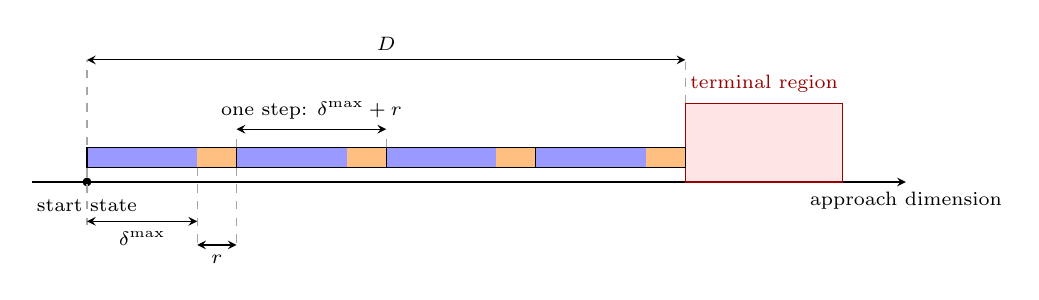
\begin{tikzpicture}[>=stealth, font=\small]
			% axis: the approach dimension
			\draw[->] (-0.3,0) -- (10.8,0)
			node[below, font=\scriptsize] {approach dimension};
			% terminal region
			\fill[red!10] (8.0,0) rectangle (10.0,1.0);
			\draw[red!60!black] (8.0,0) rectangle (10.0,1.0);
			\node[above, font=\scriptsize, red!60!black] at (9.0,1.02)
			{terminal region};
			% start state
			\fill (0.4,0) circle (1.6pt);
			\node[below, font=\scriptsize] at (0.4,-0.1) {start state};
			% distance D
			\draw[<->] (0.4,1.55) -- (8.0,1.55)
			node[midway, above, font=\scriptsize] {$D$};
			\draw[gray!70, thin, dashed] (0.4,0.05) -- (0.4,1.55);
			\draw[gray!70, thin, dashed] (8.0,1.0) -- (8.0,1.55);
			% four steps of length 1.9 = 1.4 (dynamics, blue) + 0.5 (drift, orange)
			\foreach \i in {0,1,2,3} {
				\fill[blue!40] ({0.4+\i*1.9},0.18)
				rectangle ({0.4+\i*1.9+1.4},0.44);
				\fill[orange!50] ({0.4+\i*1.9+1.4},0.18)
				rectangle ({0.4+(\i+1)*1.9},0.44);
				\draw ({0.4+\i*1.9},0.18)
				rectangle ({0.4+(\i+1)*1.9},0.44);
			}
			% labels on the first step
			\draw[gray!70, thin, dashed] (0.4,0.18) -- (0.4,-0.55);
			\draw[gray!70, thin, dashed] (1.8,0.18) -- (1.8,-0.85);
			\draw[gray!70, thin, dashed] (2.3,0.18) -- (2.3,-0.85);
			\draw[<->] (0.4,-0.5) -- (1.8,-0.5)
			node[midway, below, font=\scriptsize] {$\delta^{\max}$};
			\draw[<->] (1.8,-0.8) -- (2.3,-0.8)
			node[midway, below, font=\scriptsize] {$r$};
			% one step marked over the second segment, spanning both parts
			\draw[gray!70, thin, dashed] (2.3,0.44) -- (2.3,0.62);
			\draw[gray!70, thin, dashed] (4.2,0.44) -- (4.2,0.62);
			\draw[<->] (2.3,0.67) -- (4.2,0.67)
			node[midway, above, font=\scriptsize]
			{one step: $\delta^{\max} + r$};
		\end{tikzpicture}
		\caption{The crossing horizon, drawn for
			$k_{\text{cross}} = 4$. The start state lies at distance $D$
			from the terminal region along the approach dimension. Each
			step moves the model by at most $\delta^{\max}$ from the
			modelled dynamics (blue) plus $r$ of drift (orange). The
			fourth step reaches the terminal region.}
		\label{fig:crossing}
	\end{figure}
	
	\paragraph{Control visibility.}
	An action is useful only if the grid registers it. The model sees
	an action through the target cells its image box touches. One step
	under action $a$ displaces the image box by some amount
	$\delta_d(a)$ in each dimension $d$. A displacement smaller than
	$r_d$ in every dimension is absorbed by the per-step drift, and the
	model cannot separate taking the action from not taking it. An
	action is expressible on the grid only if
	$r_d < \lvert \delta_d(a) \rvert$ in some dimension $d$.
	
	\paragraph{Resolution against the noise.}
	In a stochastic dimension the resolution is measured against the
	noise. The stochastic factor of~\eqref{eq:mlo} and~\eqref{eq:Mhi}
	brackets the landing chance, the probability that the noisy
	coordinate lands in the target cell, over every position of the
	prediction in the image interval
	(Section~\ref{sec:abs:intervals}). When the cell width $r_d$ grows
	large against the noise spread $\sigma_d$, the landing chance
	varies from near $1$ to near $0$ as the prediction moves by one
	cell width; Figure~\ref{fig:noisewidth} draws the landing chance
	against the position of the prediction for the two cases. The
	bracket then widens towards $[0,1]$, which admits every
	probability and rules nothing out. Keeping the ratio
	$\sigma_d / r_d$ at order one or above keeps the bracket
	informative.

	\begin{figure}[h]
		\centering
		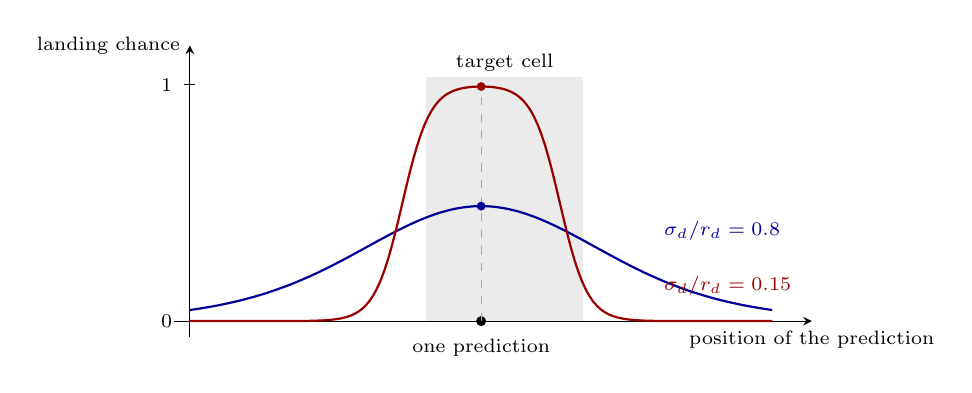
\begin{tikzpicture}[>=stealth, font=\small,
			declare function={
				phi(\x)=1/(1+exp(-1.702*max(min(\x,5),-5)));
				chance(\m,\s)=phi((2.5-\m)/\s)-phi((1.5-\m)/\s);
			}]
			% target cell band on the position axis (cell [1.5,2.5], width 1)
			\fill[black!8] (3.0,0) rectangle (5.0,3.1);
			\node[font=\scriptsize] at (4.0,3.28) {target cell};
			% axes (x: position, 1 unit = 0.5 position; y: chance, 3 = 1)
			\draw[->] (-0.2,0) -- (7.9,0)
			node[below, font=\scriptsize] {position of the prediction};
			\draw[->] (0,-0.2) -- (0,3.5)
			node[left, font=\scriptsize] {landing chance};
			\draw (-0.07,3.0) -- (0.07,3.0);
			\node[left, font=\scriptsize] at (-0.1,3.0) {$1$};
			\node[left, font=\scriptsize] at (-0.1,0) {$0$};
			% curve: cell width comparable to the noise spread
			\draw[blue!60!black, thick]
			plot[domain=0.15:3.85, samples=120]
			({2*\x-0.3}, {3*chance(\x,0.8)});
			\node[blue!60!black, font=\scriptsize, anchor=west]
			at (5.9,1.15) {$\sigma_d/r_d = 0.8$};
			% curve: cell width large against the noise spread
			\draw[red!60!black, thick]
			plot[domain=0.15:3.85, samples=160]
			({2*\x-0.3}, {3*chance(\x,0.15)});
			\node[red!60!black, font=\scriptsize, anchor=west]
			at (5.9,0.45) {$\sigma_d/r_d = 0.15$};
			% one marked prediction, at the middle of the target cell
			% (position 2.0 -> x = 3.7); chance(2.0,0.8) ~ 0.47, chance(2.0,0.15) ~ 1
			\fill (3.7,0) circle (1.8pt);
			\node[below, font=\scriptsize] at (3.7,-0.1)
			{one prediction};
			\draw[gray!70, thin, dashed] (3.7,0) -- (3.7,3.0);
			\fill[blue!60!black] (3.7,{3*chance(2.0,0.8)}) circle (1.6pt);
			\fill[red!60!black] (3.7,{3*chance(2.0,0.15)}) circle (1.6pt);
		\end{tikzpicture}
		\caption{The landing chance in one target cell (shaded) as the
			prediction moves, drawn for two ratios of noise spread to
			cell width. Each point of a curve gives the landing chance
			for a prediction at that position; one prediction at the
			middle of the target cell is marked, with its landing chance
			on each curve. With the cell width comparable to the noise
			spread (blue), the landing chance stays moderate everywhere.
			With the cell width large against the noise spread (red),
			the landing chance is near $1$ for a prediction inside the
			target cell and near $0$ one cell width away.}
		\label{fig:noisewidth}
	\end{figure}

	\paragraph{The cell budget.}
	Finer resolutions cost cells. The cell count $M$
	of~\eqref{eq:Mcount} multiplies across dimensions, and memory and
	disk cost grow with $M$, so the affordable count is capped by the
	generation infrastructure. Within the cap, a finer resolution in
	one dimension is afforded by coarsening another dimension or by
	shrinking the modelled window.
	
	\section{Case Study: An Autonomous Emergency Braking System}
	\label{sec:cs}
	
	We apply the procedure of Section~\ref{sec:abs} to a three-dimensional model of an Autonomous Emergency Braking System. Section~\ref{sec:cs:sys} describes the continuous system, Section~\ref{sec:cs:arch} the implementation architecture, Section~\ref{sec:cs:exp} the experimental configuration, the certificates, and the ten-second campaign, Section~\ref{sec:cs:horizon} the horizon-resolved campaign, Section~\ref{sec:cs:sweep} the resolution sweep, Section~\ref{sec:cs:extrafine} the second certified configuration and its results, and Section~\ref{sec:cs:future} the future work.
	
	\subsection{System description}
	\label{sec:cs:sys}
	
	\paragraph{State space.}
	The continuous state is the triple
	\begin{equation}
		s \;=\; (g,\, \vego,\, \vlead) \;\in\; \mathcal{S} \;=\; [0, 100] \times [0, 30] \times [-1, 31] \;\subset\; \R^3,
		\label{eq:statespace}
	\end{equation}
	where $g$ is the relative gap (m), $\vego$ the ego velocity (m/s), and $\vlead$ the lead velocity (m/s). The lower bound $-1$ on $\vlead$ provides one cell of headroom below zero so the discretised Gaussian tail at $\vlead = 0$ does not immediately escape the grid; physically $\vlead \ge 0$. The remaining bounds are likewise modelling choices, sized to envelope the scenarios of Section~\ref{sec:cs:exp}: velocities up to $30$\,m/s ($108$\,km/h) exceed every speed exercised there, and an initial gap of up to $100$\,m places even the fastest approach several seconds from its lead.
	
	\paragraph{Actions.}
	The controller commands one of three accelerations,
	\begin{equation}
		U \;=\; \{\,a_0 = 0,\; a_1 = -4,\; a_2 = -9.8\,\}\ \text{m/s}^2,
		\label{eq:actions}
	\end{equation}
	labelled \emph{coast}, \emph{brake}, and \emph{emergency}.
	
	\paragraph{Controller logic.}
	The controller selects among the actions of~\eqref{eq:actions} as a deterministic, memoryless function of the perceived state, through two derived quantities: the closing speed $v_{\text{rel}} = \vego - \vlead$ and the time to collision $\mathrm{TTC} = g / v_{\text{rel}}$, the latter defined when $v_{\text{rel}} > 0.1$\,m/s and taken as unbounded otherwise~\cite{EuroNCAP}. Its thresholds and decelerations are those of the implementation's \texttt{industry} configuration [CITATION FOR THE INDUSTRY BENCHMARK THRESHOLDS]. At low closing speeds ($v_{\text{rel}} < 5$\,m/s) the decision is distance-based: \emph{emergency} ($a_2$) when $g < 2$\,m, \emph{brake} ($a_1$) when $2 \le g < 6$\,m, and \emph{coast} ($a_0$) otherwise. At higher closing speeds it is TTC-based: \emph{emergency} when $\mathrm{TTC} < 1.0$\,s, \emph{brake} when $1.0 \le \mathrm{TTC} < 1.6$\,s, and \emph{coast} otherwise. An early-braking variant of the controller (\texttt{safe}), with wider thresholds and an emergency deceleration of $-8$\,m/s\textsuperscript{2}, is retained in the implementation for comparison runs and is not reported here. In the abstraction the deployed function is evaluated at cell centres and emitted as the run-length-encoded controller module of Section~\ref{sec:abs:full}.
	
	\paragraph{Terminal region and atomic propositions.}
	The designated terminal region of Section~\ref{sec:abs:partition} is $g \le 0$: transitions whose image reaches it are routed to the absorbing crash cell by Algorithm~\ref{alg:intervals}. The labels emitted with the model are predicates over the same derived quantities as the controller, evaluated at cell centres. \texttt{crash} holds on the cells whose centres satisfy $g \le 0$, that is, on the full slab of cells at the lowest gap index and not only on the absorbing cell itself; \texttt{safe} holds on every other grid cell, and \texttt{safe\_sink} on the safe sink. Two further labels mark dual-trigger risk regions, bound to the controller's warning and emergency thresholds: \texttt{braking} holds where $g < 10$\,m or $\mathrm{TTC} < 2.6$\,s, and \texttt{emergency} where $g < 2$\,m or $\mathrm{TTC} < 1.0$\,s. The label \texttt{nominal} holds on the \texttt{safe} cells outside \texttt{braking}: the states in which no braking is called for. Neither risk region coincides with the set of cells on which the controller commands the corresponding action, for two reasons: the \texttt{braking} thresholds are the warning thresholds, wider than the braking thresholds of the decision logic, and the decision logic branches on the closing speed whereas the labels apply both triggers at every state. A property over \texttt{braking} is therefore a statement about the \emph{warning region}, not about the controller braking, and a property over \texttt{emergency} is a statement about the \emph{emergency region}, not about the controller emergency-braking. The label \texttt{safe\_physics} is at present identical to \texttt{safe} and is retained for interface compatibility.
	
	\paragraph{One-step deterministic dynamics.}
	The plant computes a deterministic next state given $(s, a)$, split into an ego update, an exogenous lead update, and a gap update,
	\begin{align}
		a_{\text{ego}} &\;=\; \alpha \cdot a, \qquad \alpha = 0.5\ \text{(static actuator gain)}, \label{eq:lag}\\
		\vego' &\;=\; \max\!\bigl\{0,\; \vego + a_{\text{ego}} \cdot \dt\bigr\}, \label{eq:vego}\\
		\vlead' &\;=\; \max\!\bigl\{0,\; \vlead\bigr\} \quad \text{(default lead rule, overridable by an injected model)}, \label{eq:vlead}\\
		g' &\;=\; g + \bigl(\vlead' - \vego'\bigr) \cdot \dt, \label{eq:gap}
	\end{align}
	with $\dt = 0.1$\,s, the modelled decision period of the controller. Equation~\eqref{eq:gap} uses the updated velocities $\vego'$ and $\vlead'$ rather than their previous-step values, making this a semi-implicit (symplectic) Euler step. The ego update is controller-driven; the lead update is exogenous and does not run the controller. The factor $\alpha$ attenuates the commanded acceleration as a memoryless gain; the simulation environment implements a full first-order actuator lag, of which this stateless gain is the abstracted simplification; the value $\alpha = 0.5$ is itself a modelling choice, representing a conservatively weak actuator response.
	
	\paragraph{Monotonicity and continuity.}
	Assumption~\ref{ass:sysclass}(iii) requires each output coordinate of the one-step map to be monotone in each input coordinate, and~\eqref{eq:vego}--\eqref{eq:gap} satisfy this. $\vego'$ is nondecreasing in $\vego$ and independent of the other coordinates, the flooring $\max\{0, \cdot\}$ preserving monotonicity; $\vlead'$ is nondecreasing in $\vlead$ and independent of the others, for the same reason; and $g'$ is nondecreasing in $g$, nondecreasing in $\vlead$ through $\vlead'$, and nonincreasing in $\vego$ through $\vego'$. The extrema of every output coordinate over a cell are therefore attained at the cell's corners, as~\eqref{eq:imagebox} requires. Each output coordinate is moreover continuous in the state, the floors $\max\{0, \cdot\}$ being continuous functions, which discharges the continuity requirement of Assumption~\ref{ass:sysclass}(ii). The same floors settle the lower-boundary escape case of Section~\ref{sec:abs:intervals} for this system: $\vego'$ cannot fall below zero, and zero lies in a cell interior by the half-cell offset of~\eqref{eq:bins}, so bottom-of-grid escape does not arise in $\vego$; the gap's lower boundary is the crash wall, handled by the terminal routing; and out-of-band mass in the stochastic dimension is handled by the truncation policy, not by escape routing.
	
	\paragraph{Stochastic model.}
	The kernel is Gaussian as a consequence of the following modelling assumption.
	
	\begin{assumption}[Lead-vehicle uncertainty]
		\label{ass:lead}
		The lead-vehicle acceleration is an i.i.d.\ Gaussian random variable, $a_{\text{lead}}^{(k)} \sim \Norm(0, \sigmaa^2)$, independent across time steps. The ego dynamics and the gap update are deterministic given $(s, a)$ and the realisation of $a_{\text{lead}}^{(k)}$.
	\end{assumption}
	
	The constant $\sigmaa$ aggregates a small plant-process noise and the lead-acceleration noise,
	\begin{equation}
		\sigmaa \;=\; \sqrt{\sigma_{\text{plant}}^2 + \sigma_{\text{lead}}^2} \;=\; \sqrt{0.05^2 + 2.0^2} \;\approx\; 2.0006\ \text{m/s}^2,
		\label{eq:sigmaa}
	\end{equation}
	and a first-order Euler step on velocity gives the per-step velocity noise and the lead-velocity kernel
	\begin{equation}
		\sigmav \;=\; \sigmaa \cdot \dt \;\approx\; 0.2001\ \text{m/s}, \qquad
		\vlead' \;\sim\; \Norm\bigl(\,\max(0, \vlead),\; \sigmav^2\,\bigr).
		\label{eq:sigmav}
	\end{equation}
	The numerical values are modelling choices rather than standardised quantities: $\sigma_{\text{lead}} = 2.0$\,m/s\textsuperscript{2} is chosen so that, through~\eqref{eq:sigmav}, the lead's step-to-step speed change is moderate (a standard deviation of $0.2$\,m/s per $0.1$\,s step), and $\sigma_{\text{plant}} = 0.05$\,m/s\textsuperscript{2} is a small allowance for unmodelled plant disturbance; neither is calibrated against measured driving data at this stage of the programme.
	
	\begin{remark}[Process noise is prediction uncertainty, not estimation uncertainty]
		The Gaussian term in~\eqref{eq:sigmav} models what the lead vehicle will do
		over the coming time step, not how accurately the current state is measured.
		The kernel mean $\max(0, \vlead)$ is the lead model's deterministic
		prediction of the next lead velocity, and the scatter around it is the
		effect of the lead acceleration of Assumption~\ref{ass:lead}, which at the
		moment of prediction has not yet been realised. Under the perfect-perception
		setting of this paper the current state $(g, \vego, \vlead)$ is known
		exactly; the uncertainty concerns its evolution, and no sensor fidelity
		reduces it, since a sensor reports the lead's present velocity rather than
		its driver's next decision. It is therefore distinct from, and orthogonal
		to, the perception uncertainty of the later tracks
		(Section~\ref{sec:cs:future}), which concerns errors in estimating the
		current state; the perception-aware construction composes the two rather
		than substituting one for the other.
	\end{remark}
	
	\paragraph{The gap-noise approximation.}
	Since $g' = g + (\vlead' - \vego')\,\dt$ and $\vlead'$ is the only random input, $g'$ inherits noise from $\vlead'$: the true joint distribution of $(g', \vlead')$ is a degenerate (rank-one) bivariate Gaussian, with
	\begin{equation}
		\sigma_g \;=\; \sigmav \cdot \dt \;\approx\; 0.02\ \text{m}.
		\label{eq:gapnoise}
	\end{equation}
	We discard this correlation and treat $g$ as deterministic given the centroid. This is a deliberate simplification: with cell width of order $1$\,m and $\sigma_g \approx 0.02$\,m, a single Gaussian step in gap is well within one cell, and the simplification keeps the kernel factorisable as a product of marginals across dimensions. The implementation reflects this by setting $\sigma_{\text{per dim}} = (0,\, 0,\, \sigmav)$. The containment certificate of Section~\ref{sec:abs:sound} is evaluated against this same modelling kernel.
	
	\paragraph{Kernel structure.}
	The modelling kernel is therefore a product of three one-dimensional
	factors, discharging the factorisation requirement of
	Assumption~\ref{ass:sysclass}(i): Dirac point masses on gap and $\vego$,
	whose one-step values are computed exactly by~\eqref{eq:vego}
	and~\eqref{eq:gap}, and a Gaussian density on $\vlead$, given
	by~\eqref{eq:sigmav}. Figure~\ref{fig:kernelfactors}
	traces one step: the transition probability to a target cell is the product
	of two indicator factors and one area factor. This is the concrete instance
	of the generic factor split of Section~\ref{sec:abs:intervals}
	(Figure~\ref{fig:atomvsdensity}), and it delimits where the ingredients of
	Section~\ref{sec:abs:rel} apply: the range bound of~\cite{Soudjani2013}
	operates on the density factor, and the image-box enumeration on the two
	point-mass factors.
	
	\begin{figure}[h]
		\centering
		\resizebox{0.98\textwidth}{!}{%
			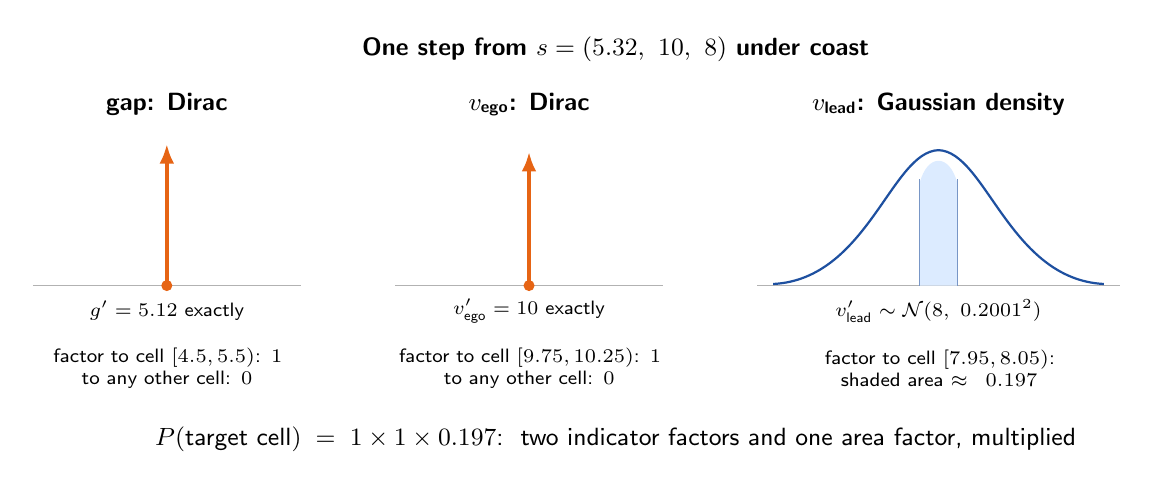
\begin{tikzpicture}
				\node[font=\small\sffamily\bfseries] at (7.6,3.6)
				{One step from $s = (5.32,\ 10,\ 8)$ under \emph{coast}};
				% panel 1: gap
				\node[font=\small\sffamily\bfseries] at (1.9,2.9) {gap: Dirac};
				\draw[gray!60] (0.2,0.6) -- (3.6,0.6);
				\draw[accentOrange, ultra thick, -{Latex[length=2.5mm]}] (1.9,0.6) -- (1.9,2.4);
				\fill[accentOrange] (1.9,0.6) circle (2pt);
				\node[font=\scriptsize\sffamily] at (1.9,0.28) {$g' = 5.12$ exactly};
				\node[font=\scriptsize\sffamily, text width=3.3cm, align=center] at (1.9,-0.45)
				{factor to cell $[4.5, 5.5)$: $1$\\to any other cell: $0$};
				% panel 2: v_ego
				\begin{scope}[shift={(4.6,0)}]
					\node[font=\small\sffamily\bfseries] at (1.9,2.9) {$\vego$: Dirac};
					\draw[gray!60] (0.2,0.6) -- (3.6,0.6);
					\draw[accentOrange, ultra thick, -{Latex[length=2.5mm]}] (1.9,0.6) -- (1.9,2.3);
					\fill[accentOrange] (1.9,0.6) circle (2pt);
					\node[font=\scriptsize\sffamily] at (1.9,0.28) {$\vego' = 10$ exactly};
					\node[font=\scriptsize\sffamily, text width=3.3cm, align=center] at (1.9,-0.45)
					{factor to cell $[9.75, 10.25)$: $1$\\to any other cell: $0$};
				\end{scope}
				% panel 3: v_lead
				\begin{scope}[shift={(9.2,0)}]
					\node[font=\small\sffamily\bfseries] at (2.5,2.9) {$\vlead$: Gaussian density};
					\draw[gray!60] (0.2,0.6) -- (4.8,0.6);
					\fill[imdpLightBlue] (2.26,1.9) .. controls (2.36,2.28) and (2.64,2.28) .. (2.74,1.9)
					-- (2.74,0.6) -- (2.26,0.6) -- cycle;
					\draw[imdpBlue, thick] (0.4,0.62) .. controls (1.6,0.68) and (1.9,2.3) .. (2.5,2.32)
					.. controls (3.1,2.3) and (3.4,0.68) .. (4.6,0.62);
					\draw[imdpBlue!60] (2.26,0.6) -- (2.26,1.95);
					\draw[imdpBlue!60] (2.74,0.6) -- (2.74,1.95);
					\node[font=\scriptsize\sffamily] at (2.5,0.28) {$\vlead' \sim \Norm(8,\ 0.2001^2)$};
					\node[font=\scriptsize\sffamily, text width=4.4cm, align=center] at (2.5,-0.45)
					{factor to cell $[7.95, 8.05)$: shaded area $\approx 0.197$};
				\end{scope}
				\node[font=\small\sffamily] at (7.6,-1.35)
				{$P(\text{target cell}) \;=\; 1 \times 1 \times 0.197$:\ \ two indicator
					factors and one area factor, multiplied};
			\end{tikzpicture}%
		}
		\caption{The AEBS modelling kernel as a product of three one-dimensional
			factors, traced for one step. The deterministic dimensions carry Dirac
			point masses (indicator factors); the lead velocity carries a Gaussian
			density (an area factor). The probabilities shown are exact for the
			\code{medium\_tight} grid of Section~\ref{sec:cs:exp}.}
		\label{fig:kernelfactors}
	\end{figure}
	
	\paragraph{Lead-behaviour model.}
	The exogenous lead rule of~\eqref{eq:vlead} is supplied by an injectable lead-behaviour model, which owns the lead's dynamics and their modelling envelope: the transition rule, the noise level of Assumption~\ref{ass:lead}, and the grid band of the stochastic dimension. One deterministic profile is composed at present, implementing the hold rule of~\eqref{eq:vlead}: the lead's next velocity is its current velocity, floored at zero. A stationary lead and a constant-speed lead are both instances of this rule, distinguished only by the initial lead velocity; both correspond to standard car-to-car rear test scenarios~\cite{EuroNCAP}. Verification scenarios are not properties of the lead model: they are start states of the encounter, specified by the ego's situation at time zero in continuous coordinates and resolved to grid cells (Section~\ref{sec:cs:exp}), so one scenario catalogue serves any lead profile whose grid band contains its states. With a moving lead the gap update couples to the lead velocity, which shears the image set of each source cell and widens the deterministic gap bracket relative to the stationary case; this affects the tightness of the intervals, not their soundness. A nondeterministic lead, which may apply any of a set of admissible accelerations at each step~\cite{EuroNCAP}, is defined in the implementation but not composed: it requires a second (lead) action axis in the discretiser and the composition, and its treatment is deferred to Section~\ref{sec:cs:future}.
	
	\paragraph{Formal classification.}
	With a deterministic lead, the system is a discrete-time stochastic control system $\Sigma = (\mathcal{X}, U, T_x)$ in the sense of~\cite[Sec.~3]{Soudjani2013}, with $\mathcal{X}$ continuous, $U$ finite, and $T_x$ a Dirac--Gaussian product kernel; the controller's operating regimes are values of the input $a \in U$, not discrete plant modes, so $|Q| = 1$ and the full hybrid-mode machinery of~\cite[Sec.~4]{Soudjani2013} is not needed. The restriction to $|Q| = 1$ is a property of the present closed loop, not of the construction: because the plant rows depend only on the cell and the commanded acceleration, a controller with a persistent internal mode, for instance a supervisor toggling between the deployed law and a fallback law, would make the composed system a stochastic hybrid system with $|Q| \ge 2$ while reusing this plant IMDP and its containment certificate unchanged (Section~\ref{sec:abs:rel}). The runtime monitors envisaged by the wider programme, which may switch to a fallback law on detecting a perception failure, are supervisors of exactly this kind. A nondeterministic lead would introduce a second action axis, over which the model checker would quantify in the worst case; building that path is the deferred extension.
	
	\subsection{Implementation architecture}
	\label{sec:cs:arch}
	
	The case-study system comprises four logical subsystems (Figure~\ref{fig:arch}): two perception components that consume camera and radar inputs, a controller that fuses their outputs and selects an action, and a vehicle plant whose continuous dynamics produce the next state. Under perfect perception the perception components are exact, and only the plant is abstracted; the perception and controller subsystems are exact symbolic translations into PRISM.
	
	\begin{figure}[h]
		\centering
		\resizebox{0.9\textwidth}{!}{%
			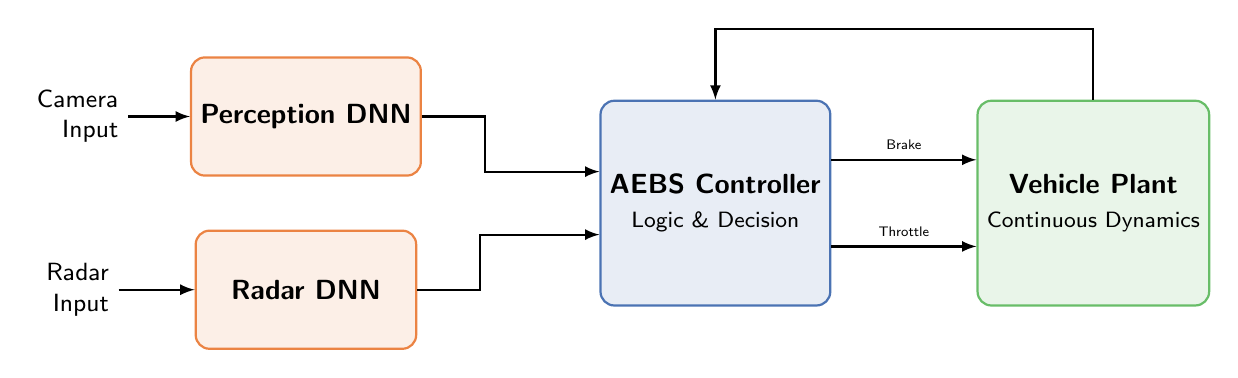
\begin{tikzpicture}[
				arch_dnn/.style    = {draw=accentOrange!80, rectangle, rounded corners=5pt, thick,
					minimum height=1.7cm, minimum width=2.8cm, align=center,
					fill=accentOrange!10, font=\sffamily},
				arch_ctrl/.style   = {draw=imdpBlue!80, rectangle, rounded corners=5pt, thick,
					minimum height=3.6cm, minimum width=2.8cm, align=center,
					fill=imdpBlue!10, font=\sffamily},
				arch_plant/.style  = {draw=safeGreen!70, rectangle, rounded corners=5pt, thick,
					minimum height=3.6cm, minimum width=2.8cm, align=center,
					fill=safeGreen!10, font=\sffamily},
				line/.style        = {->, thick, >=latex, font=\scriptsize\sffamily}
				]
				\node[arch_dnn, minimum height=1.5cm, minimum width=2.8cm]
				(dnn1) at (0, 1.1) {\textbf{Perception DNN}};
				\node[arch_dnn, minimum height=1.5cm, minimum width=2.8cm]
				(dnn2) at (0, -1.1) {\textbf{Radar DNN}};
				\node[arch_ctrl, minimum height=2.6cm, minimum width=2.8cm]
				(ctrl) at (5.2, 0) {\textbf{AEBS Controller}\\\footnotesize Logic \& Decision};
				\node[arch_plant, minimum height=2.6cm, minimum width=2.8cm]
				(plant) at (10.0, 0) {\textbf{Vehicle Plant}\\\footnotesize Continuous Dynamics};
				
				\node[font=\small\sffamily, align=right] (img_in) at (-2.9, 1.1) {Camera\\Input};
				\node[font=\small\sffamily, align=right] (rad_in) at (-2.9, -1.1) {Radar\\Input};
				\draw[thick,->,>=latex] (img_in) -- (dnn1);
				\draw[thick,->,>=latex] (rad_in) -- (dnn2);
				
				\draw[line] (dnn1.east) -- ++(0.8,0) |- ([yshift=0.40cm]ctrl.west);
				\draw[line] (dnn2.east) -- ++(0.8,0) |- ([yshift=-0.40cm]ctrl.west);
				\draw[line] ([yshift=0.55cm]ctrl.east) -- node[above,font=\tiny\sffamily]{Brake} ([yshift=0.55cm]plant.west);
				\draw[line] ([yshift=-0.55cm]ctrl.east) -- node[above,font=\tiny\sffamily]{Throttle} ([yshift=-0.55cm]plant.west);
				\draw[line] (plant.north) -- ++(0,0.9) -| (ctrl.north);
			\end{tikzpicture}%
		}
		\caption{Case-study system architecture. Under perfect perception only the plant is abstracted.}
		\label{fig:arch}
	\end{figure}
	
	The PRISM encoding comprises four modules, synchronised by a small scheduler.
	
	\begin{center}
		\begin{tabular}{ll}
			\toprule
			\textbf{Module} & \textbf{Responsibility} \\
			\midrule
			Plant (IMDP) & Stochastic physics; built by discretisation. \\
			Perception (deterministic) & Identity in perfect perception; optional sensor noise otherwise. \\
			Controller (deterministic) & Symbolic action selection; one rule per cell, run-length encoded. \\
			Turn (scheduler) & Enforces order $\texttt{perceive} \to \texttt{control} \to \texttt{time\_step}$. \\
			\bottomrule
		\end{tabular}
	\end{center}
	\subsection{Experimental configuration, certificates, and verification}
	\label{sec:cs:exp}
	
	\paragraph{Configuration.}
	We report the \code{medium\_tight} grid preset, the configuration on which the abstraction is certified, with the deterministic lead started stationary. The grid shape is $(101, 61, 321)$, giving $M = 1{,}977{,}681$ cells.
	
	\begin{center}
		\begin{tabular}{ll}
			\toprule
			\textbf{Parameter} & \textbf{Value} \\
			\midrule
			Grid resolution $(r_g, r_{\vego}, r_{\vlead})$ & $(1.0,\,0.5,\,0.1)$ \\
			Bounds $(g, \vego, \vlead)$ & $[0,100]\times[0,30]\times[-1,31]$ \\
			Grid shape $(n_g, n_{\vego}, n_{\vlead})$ & $(101,\,61,\,321)$ \\
			Number of cells $M$ & $1{,}977{,}681$ \\
			Lead-acceleration std $\sigmaa$ & $\approx 2.0006$ m/s\textsuperscript{2} (Eq.~\ref{eq:sigmaa}) \\
			Velocity-step std $\sigmav$ & $\approx 0.2001$ m/s (Eq.~\ref{eq:sigmav}) \\
			Time step $\dt$ & $0.1$ s \\
			Action set $U$ & $\{0, -4, -9.8\}$ m/s\textsuperscript{2} (Eq.~\ref{eq:actions}) \\
			Controller configuration & \texttt{industry} \\
			Lead model & hold rule, deterministic~\cite{EuroNCAP} \\
			Stochastic-tail policy & truncating; renormalised within the grid band (Eq.~\ref{eq:trunc}) \\
			\bottomrule
		\end{tabular}
	\end{center}
	
	The state count reflects the choice of $r_{\vlead} = 0.1$ m/s, which is half the velocity-step noise standard deviation $\sigmav$, giving a noise-to-cell-width ratio of $\sigmav / r_{\vlead} \approx 2.0$. This is at the lower end of what keeps the range-based factor~\eqref{eq:Mm} non-degenerate; the resolution is essentially as coarse as it can be taken without the stochastic factor collapsing.
	
	\paragraph{Containment certificate.}
	The containment test of Section~\ref{sec:abs:sound} is run over the entire \code{medium\_tight} grid. It visits every one of the $M = 1{,}977{,}681$ source cells under all three actions and samples $3$ states per dimension, $27$ per cell, spanning the half-open extent of the cell: in each dimension the samples run from the exact lower edge to the largest floating-point value strictly below the upper edge. At each sampled state it checks that the true one-step transition probability to each reachable target cell lies within the stored interval, at a numerical tolerance of $10^{-7}$. The tolerance dominates the only mass the construction deliberately neglects, the Gaussian tail beyond the $\pm 6\sigmav$ search window and the dropped negligible products of Section~\ref{sec:abs:intervals}, both of order $10^{-9}$ or below. Certificates are bound to a \emph{run identity} comprising the lead model, the grid preset, the partition fingerprint (a hash of the exact cell edges; here \code{3672963e58eb75b5}), a hash of the kernel source, the controller configuration together with its action values, and the test version; progress recorded under one identity cannot be resumed under another, so a certificate can never silently mix configurations. For the configuration of this section the test visited all $1{,}977{,}681$ cells under all three actions, processed in $989$ chunks on $32$ cores of the cluster node, and completed with \emph{zero} violations and a worst recorded excess of $0$; the run identity is \code{static\_industry\_medium\_tight\_g3672963e\_ka6a68d63\_abb83a370\_v3}, at code revision \code{3b9f3e9}, and the run completed in under $65$ minutes of wall-clock time. This discharges the containment hypothesis~\eqref{eq:containment} for the reported configuration and, together with the robust-verification argument of Section~\ref{sec:abs:sound}, certifies the abstraction as a sound over-approximation of the modelling kernel.
	
	\paragraph{Interval-width diagnostic.}
	The diagnostic~\eqref{eq:Edef} was computed on the assembled production IMDP: the worst-row half-width sum is $K = 6.276171$, giving $E = N \cdot K = 62.761707$ at the reporting horizon $N = 10$, attained by a \emph{coast} row in the topmost $\vlead$ band of the grid. A bound of this magnitude on a probability is vacuous, as anticipated structurally in Sections~\ref{sec:rw} and~\ref{sec:abs:sound}: with state-independent noise the per-row width is essentially uniform across the state space, and the maximising rows sit where the truncation renormalisation of~\eqref{eq:trunc} divides by the smallest in-band Gaussian mass, at the edge of the grid band. The containment certificate above is unaffected; $E$ plays no role in it.
	
	\paragraph{Structure of the interval lower bounds.}
	The deterministic factor~\eqref{eq:flo} contributes its certain value only when the image interval lies strictly inside a single half-open target cell, and for this system that containment never holds on an interior cell. In the gap dimension the image of a cell is the cell's own width plus the shear contributed by the velocity coupling of~\eqref{eq:gap}, so it is strictly wider than one cell; in the $\vego$ dimension the image is a translation of the cell by $a_{\text{ego}} \cdot \dt$, of exactly the cell's width, which fails the strict upper inequality of~\eqref{eq:flo} even when the translation aligns with the grid. Every interior transition therefore carries the lower bound $0$, at every grid resolution; refinement does not remove this. Each such bound is exact rather than conservative: for a straddled target, some state of the source cell reaches it with probability $0$, so $0$ is the true minimum of~\eqref{eq:txonstates} over the cell. The looseness of the abstraction lies instead in the independence of the per-target intervals: the stored constraints bound each target separately, together with row feasibility, and discard the fact that all states of a cell follow a single one-step distribution. The effect on the verified values is bounded by the row's upper bounds, which confine every admissible distribution to the block of target cells the image box touches; the freedom the zero lower bounds grant therefore amounts to a displacement of at most one cell width per step around the modelled dynamics. Refining the grid shrinks that displacement in physical units and narrows the verified brackets, although the per-transition zeros persist. The pair $[P_{\min}, P_{\max}]$ is reported as a bracket whose width is the abstraction's precision at the property's horizon: the displacement budget grows by one cell width per period, so the brackets are informative only at horizons over which the accumulated budget remains small against the distances that decide the property.
	
	\paragraph{Model generation.}
	Generating the model at this resolution exceeds the memory of the development workstation: the image-box kernel produces several times more transitions per row than a single-target routing would. Production generation is therefore performed on a departmental cluster node with $64$ cores and $503$\,GB of memory, parallelised over $63$ worker processes; the partition fingerprint recorded at generation is required to match that of the containment certificate. Both exporters print every interval bound to eight decimal places, rounded outward: lower bounds are rounded down and upper bounds up, clamped to $[0,1]$. Outward rounding widens a printed interval by at most one quantum of $10^{-8}$, and a widened interval that contained the true transition probability still contains it, so the printed model inherits the containment property of the in-memory intervals; the quantisation is two orders of magnitude below the certificate tolerance. For the configuration of this section, generation completed in approximately $43$ minutes of wall-clock time, producing a modular PRISM artifact of $31{,}073{,}746{,}675$ bytes (approximately $28.9$\,GiB) and a direct-encoding artifact of $11{,}002{,}523{,}700$ bytes (approximately $10.2$\,GiB), at code revision \code{3b9f3e9}.
	
	\paragraph{Model checking at scale.}
	Storm's PRISM engine parses a model file into an in-memory syntactic representation before constructing the state space, and at the size of the production artifact that representation exceeded the memory of the cluster node: seven per-scenario invocations against the modular PRISM file were terminated by the operating system after $2.5$ to $3.4$ hours each, returning no results. The pipeline therefore emits, alongside the modular PRISM model, the same abstraction in Storm's \emph{direct encoding} (DRN)~\cite{Storm}: an explicit listing of states, actions, interval transitions, and state labels that the checker streams directly into its sparse model representation, with no syntactic intermediate. The direct encoding has no module or synchronisation syntax, so the object emitted in it is the flattened synchronised product of the modular model, which is in any case the object Storm itself constructs when checking the modular file.
	
	Under perfect perception the product admits an exact reduction. Write $C(c_i)$ for the quantised controller of Section~\ref{sec:abs:full}, the action assigned to state $i$ at its centre. In the modular model one \emph{control period}, of duration $\dt$, consists of three synchronised transitions: \texttt{perceive} copies the plant state to the controller's input, \texttt{control} applies the controller function to that input, and \texttt{time\_step} draws the next plant state from the row of the current state under the commanded action. The first two transitions are deterministic, so the action commanded at plant state $i$ is $C(c_i)$ in every period, and the product reduces to the \emph{closed-loop} IMDP over the plant's own states, carrying a single action per state:
	\begin{equation}
		\hat U_{\mathrm{cl}}(i) \;=\; \{\, C(c_i) \,\}, \qquad
		\check P_{\mathrm{cl}}(i, \cdot) = \check P\bigl(i, C(c_i), \cdot\bigr), \qquad
		\hat P_{\mathrm{cl}}(i, \cdot) = \hat P\bigl(i, C(c_i), \cdot\bigr),
		\label{eq:collapse}
	\end{equation}
	where $\check P, \hat P$ are the plant intervals of~\eqref{eq:imdp} and the subscript marks the closed-loop model. The reduction changes the step accounting: one transition of the closed-loop encoding is one control period, whereas one period costs three transitions of the modular model. A bounded-reachability horizon of $N$ periods is therefore expressed as a step bound of $N$ on the closed-loop encoding and of $3N$ on the modular model; property step bounds are not interchangeable between the two.
	
	\paragraph{Equivalence certificate.}
	The closed-loop encoding is produced by a separate exporter, so its agreement with the modular model is checked file against file rather than assumed. The check first parses the modular file's perception module and fails unless it is the symbolic identity, the validity condition of the reduction~\eqref{eq:collapse}; it then parses the run-length-encoded controller module into the full map $i \mapsto C(c_i)$. It then verifies, streaming both files in lockstep: that the closed-loop encoding carries exactly one action per state; that this action equals $C(c_i)$; that its transition list equals the plant row of $(i, C(c_i))$ in the modular file, target for target and bound for bound; and that the label state sets of the two files coincide. A cryptographic hash of the compared transition stream is recorded on both sides as the certificate of a passing run. The reduction is additionally validated numerically: on a coarse grid of $11{,}088$ cells, the bounded-reachability values of the modular model at step bound $3k$ and of the closed-loop encoding at step bound $k$ agree to within $10^{-12}$ for $k$ up to $100$, under both the worst-case and the best-case interval resolution. For the production artifacts the check passed: the direct encoding carries exactly one action per state across all $1{,}977{,}682$ states (the grid cells and the safe sink), every transition list matches the controller-selected plant row bound for bound, and the label state sets of the two files coincide, with the scenario labels present only in the direct encoding as intended, in approximately $31$ minutes of wall-clock time; the canonical hash \code{052370659bd5733e512f2175a93f7d075b8faa2751232452adfa1d21d45fe6c3} was recorded identically for the composed modular model and the direct encoding.
	
	\paragraph{Scenario states.}
	The verification campaign addresses four non-absorbing scenario states, staged points along a car-to-car rear encounter with a stationary lead (the CCR scenario family of~\cite{EuroNCAP}), together with one state inside the terminal region used as a sanity check; Table~\ref{tab:scenarios} lists them. The scenarios are specified by the ego's situation at time zero, in continuous coordinates, and each resolves to the cell of the \code{medium\_tight} grid whose centre is the stated state; the resolved identifiers are functions of the partition fingerprint alone. The action column records the controller decision at the cell centre under the logic of Section~\ref{sec:cs:sys}; the scenario names describe the staging of the encounter, not that decision. In the closed-loop encoding each scenario state additionally carries a dedicated state label, and the region labels of Section~\ref{sec:cs:sys} are carried by both encodings, so that scenarios and regions are addressable by the verifier without external state identifiers.
	
	\begin{table}[h]
		\centering
		\begin{tabular}{lllr}
			\toprule
			Scenario & $(g, \vego, \vlead)$ & Action & State id \\
			\midrule
			Safe\_Cruising & $(100,\ 15,\ 0)$ & coast & 1967740 \\
			Warning\_Brake & $(30,\ 7,\ 0)$ & coast & 591934 \\
			Emergency\_Brake & $(10,\ 10,\ 0)$ & brake & 202240 \\
			Imminent\_Collision & $(5,\ 30,\ 0)$ & emergency & 117175 \\
			Post\_Collision & $(0,\ 0,\ 0)$ & (terminal region) & 10 \\
			\bottomrule
		\end{tabular}
		\caption{Scenario states on the \code{medium\_tight} grid under the \texttt{industry} controller. Post\_Collision lies inside the terminal region, so its bounded-reachability value must be exactly $1$; it is verified as an end-to-end sanity check of the emitted model rather than as a scenario of interest.}
		\label{tab:scenarios}
	\end{table}
	
	\paragraph{Verification.}
	For each non-absorbing scenario state of Table~\ref{tab:scenarios} we compute the bounded-reachability interval $[P_{\min}, P_{\max}]$ for reaching a crash within a horizon of $N = 100$ control periods ($10$\,s at $\dt = 0.1$\,s), expressed against the closed-loop encoding as \code{F<=100 "crash"}. Robust verification is performed with Storm~1.13.0~\cite{Storm} (official container build, Z3 backend), which recognises the encoding as an interval MDP and applies robust value iteration under the worst-case (for $P_{\max}$) and best-case (for $P_{\min}$) resolution of the intervals. On the production artifact Storm constructs the sparse model in approximately $768$\,s; the constructed model has $1{,}977{,}682$ states, one choice per state, confirming the closed-loop structure of~\eqref{eq:collapse}, and $307{,}323{,}579$ interval transitions. One value iteration computes the value at every state simultaneously, so all properties of one resolution are evaluated in a single invocation that parses the model once; individual scenario states and whole regions are then read off with property filters over the state labels, for example
	\begin{center}
		\code{filter(max, Pmax=?\ [ F<=100 "crash" ], "nominal")}.
	\end{center}
	A filtered maximum over a region label is the largest worst-case value over every start state carrying the label. Over \texttt{nominal} it is the statement \emph{starting anywhere with no need to brake, the probability of a crash within $10$\,s is at most the reported value}; the corresponding filtered minimum under the best-case resolution completes the bracket. The same properties over \texttt{braking} and \texttt{emergency} are statements about the warning region and the emergency region respectively, in the sense fixed in Section~\ref{sec:cs:sys}. The Post\_Collision filter is the sanity check, required to return exactly $1$. The maximise batch completed in $10{,}115.606$\,s of wall-clock time with a peak memory of $37{,}515$\,MB, as reported by the checker's own resource measurement; the minimise batch completed in $5{,}923.478$\,s at a peak of $37{,}518$\,MB.
	\paragraph{Results.}
	Table~\ref{tab:results} reports the campaign. Three observations follow. First, the sanity check passes: the Post\_Collision state, inside the terminal region, returns exactly $1$. Second, the Imminent\_Collision bracket is $[1, 1]$: every transition distribution consistent with the certified intervals reaches a crash within the horizon, so by the argument of Section~\ref{sec:abs:sound} the modelled system crashes from that state with probability exactly $1$. The result is physically expected: the scenario closes at $30$\,m/s over a $5$\,m gap, while the strongest response the plant can realise, the emergency action through the actuator gain of~\eqref{eq:lag}, has a stopping distance of roughly $92$\,m. Third, every other bracket is $[0, 1]$, the vacuous interval, and this is the saturation anticipated by the displacement-budget analysis of Section~\ref{sec:abs:budget}: the intervals admit a drift of up to one gap cell, $1$\,m, per period, so over $100$ periods the budget spans the entire $100$\,m gap axis, letting the worst-case resolution reach the crash wall from every reported start state and the best-case resolution avoid it from every reported start state except Imminent\_Collision. The saturated brackets are sound and carry information about the abstraction rather than the system: at this resolution, the ten-second horizon exceeds what the intervals can decide. Two experiments follow directly: computing the brackets as functions of the step bound, which locates the largest horizon this resolution decides (Section~\ref{sec:cs:horizon}), and refining the grid over a reduced window (Section~\ref{sec:cs:extrafine}).
	
	\begin{table}[h]
		\centering
		\begin{tabular}{llcc}
			\toprule
			Start set & Kind & $P_{\min}$ & $P_{\max}$ \\
			\midrule
			Safe\_Cruising & scenario state & $0$ & $1$ \\
			Warning\_Brake & scenario state & $0$ & $1$ \\
			Emergency\_Brake & scenario state & $0$ & $1$ \\
			Imminent\_Collision & scenario state & $1$ & $1$ \\
			Post\_Collision & sanity check & --- & $1$ \\
			\texttt{nominal} & region & $0$ & $1$ \\
			\texttt{braking} (warning region) & region & $0$ & $1$ \\
			\texttt{emergency} (emergency region) & region & $0$ & $1$ \\
			\bottomrule
		\end{tabular}
		\caption{Bounded-reachability results for \code{F<=100 "crash"} ($10$\,s at $\dt = 0.1$\,s) on the certified closed-loop encoding. Scenario rows report the bracket at the single labelled state. Region rows report the envelope over the region: the smallest best-case value and the largest worst-case value over every start state carrying the label. Post\_Collision is the sanity check of Table~\ref{tab:scenarios}, evaluated under the worst-case resolution only. Values are exactly as reported by the checker. Provenance: partition fingerprint \code{3672963e58eb75b5}, code revision \code{3b9f3e9}, containment run identity and equivalence certificate of this section.}
		\label{tab:results}
	\end{table}
	\subsection{Horizon-resolved verification on the production grid}
	\label{sec:cs:horizon}
	
	The saturation of Table~\ref{tab:results} is horizon-dependent, so we query the same certified model at a ladder of step bounds, the \emph{horizon rungs}
	\begin{equation}
		k \;\in\; \{5,\ 10,\ 15,\ 20,\ 25,\ 30,\ 40,\ 50,\ 75\};
		\label{eq:rungs}
	\end{equation}
	\emph{rung spacing} denotes the difference between successive queried bounds. Each rung is one property \code{F<=k "crash"} against the certified closed-loop encoding of Section~\ref{sec:cs:exp}; one Storm invocation evaluates a batch of rungs after constructing the model once.
	
	Table~\ref{tab:frontier} reports the frontier. Three findings. First, $P_{\max}$ transitions from $0$ to $1$ within a single rung for every start set at this spacing, so the decidable horizon is located to one rung. Second, $P_{\min} = 0$ at all $36$ start-set and rung combinations, as the structural analysis of Section~\ref{sec:cs:exp} predicts; the zero lower bounds are horizon-resolved, not an artefact of the ten-second query. Third, the ordering of the crossings follows the distance to the terminal region, consistent with the budget rule of Section~\ref{sec:abs:budget}.
	
	\begin{table}[h]
		\centering
		\begin{tabular}{lcc}
			\toprule
			Start set & last rung with $P_{\max} = 0$ & first rung with $P_{\max} = 1$ \\
			\midrule
			Emergency\_Brake & $5$ & $10$ \\
			Warning\_Brake & $15$ & $20$ \\
			Safe\_Cruising & $30$ & $40$ \\
			\texttt{nominal} (region) & $5$ & $10$ \\
			\bottomrule
		\end{tabular}
		\caption{Horizon-resolved frontier on the production grid (\code{medium\_tight}), rungs as in~\eqref{eq:rungs}. Every measured transition is $0 \to 1$ within one rung; no intermediate value was observed at this spacing. $P_{\min} = 0$ at all $36$ combinations. Imminent\_Collision is $[1,1]$ from the first rung onwards and is omitted. Provenance as in Table~\ref{tab:results}.}
		\label{tab:frontier}
	\end{table}
	
	Provenance and cost. The maximise batch terminated early after $21$ of $36$ properties; the three affected cells (Safe\_Cruising at $k \in \{40, 50, 75\}$) were recovered by a separate invocation, and every value in Table~\ref{tab:frontier} has a checker log line. $P_{\max}$ cells above a measured value of $1$ are implied by monotonicity of $P_{\max}$ in $k$ and were not re-run. Model construction from the direct encoding costs approximately $710$\,s per invocation; per-property checking time grows approximately linearly in $k$, from $65$\,s at $k = 5$ to $787$\,s at $k = 75$. The minimise batch ($36$ properties) completed in $7{,}926.832$\,s at a peak of $37{,}516$\,MB; the recovery invocation completed in $2{,}229.7$\,s at a peak of $37{,}514$\,MB.
	
	The frontier sharpens the reading of Table~\ref{tab:results}: the production resolution decides Warning\_Brake safety to $1.5$\,s and Safe\_Cruising safety to $3$\,s, and returns no fractional value anywhere. Locating fractional brackets requires finer resolution; the next two subsections report where and how.
	
	\subsection{Resolution sweep}
	\label{sec:cs:sweep}
	
	Four exploratory grids isolate the effect of resolution. All use the kernel, controller, and lead of Section~\ref{sec:cs:exp} over a reduced window, $g \in [0, 100]$, $\vego \in [0, 16]$, $\vlead \in [-1, 3]$; Imminent\_Collision lies outside this window by design, its bracket being already decided as $[1,1]$ on the production grid. Each sweep grid passed the file-against-file equivalence check of Section~\ref{sec:cs:exp} before verification. The sweep grids carry \emph{no} containment certificate: their measurements are methodology evidence for the rules of Section~\ref{sec:abs:budget}, and only the two certified configurations ship results.
	
	\begin{table}[h]
		\centering
		\begin{tabular}{lll}
			\toprule
			Preset & $(r_g,\ r_{\vego},\ r_{\vlead})$ & Role \\
			\midrule
			\code{r100} & $(1.0,\ 0.5,\ 0.1)$ & production resolution, reduced window \\
			\code{r050} & $(0.5,\ 0.5,\ 0.1)$ & gap halved \\
			\code{r025} & $(0.25,\ 0.5,\ 0.1)$ & gap quartered \\
			\code{r050v} & $(0.5,\ 0.25,\ 0.1)$ & ego halved (control-visibility probe) \\
			\bottomrule
		\end{tabular}
		\caption{Sweep presets. Window $g \in [0, 100]$, $\vego \in [0, 16]$, $\vlead \in [-1, 3]$ throughout; equivalence-checked, not containment-certified.}
		\label{tab:sweeps}
	\end{table}
	
	Three measurements follow.
	\begin{enumerate}
		\item \emph{Crossings move outward with gap resolution.} From \code{r100} to \code{r050}: Warning\_Brake $15 \to 20$, Safe\_Cruising $40 \to 50$, \texttt{nominal} $5 \to 10$. From \code{r050} to \code{r025} the crossings are unchanged at $5$-step rung spacing. The first fractional certificate of the study appears here: $P_{\max} = 0.9846419946$ for Safe\_Cruising at $k = 50$ on \code{r050}.
		\item \emph{Finer rungs sharpen the frontier.} At $1$--$2$ step rung spacing, Safe\_Cruising transitions between $48$ and $52$ on \code{r050} and between $55$ and $60$ on \code{r025}; Warning\_Brake transitions between $21$ and $23$ on \code{r050} and between $23$ and $25$ on \code{r025}, with $P_{\max} = 0.9999807082$ at $k = 25$. The apparent one-rung walls of Table~\ref{tab:frontier} are a property of the rung spacing, and gap refinement pays with diminishing returns.
		\item \emph{The ego probe confirms the control-visibility rule.} On \code{r050v}, with $r_{\vego} = 0.25$ below the emergency threshold of $0.49$\,m/s, Safe\_Cruising returns the fractional certificate $P_{\max} = 0.999865419$ at $k = 52$, a rung at which \code{r050} ($r_{\vego} = 0.5$, both thresholds failed) has already saturated at $1$. Finer ego resolution makes the emergency response visible to the grid and removes part of the worst case available at the coarser ego resolution.
	\end{enumerate}
	The linear budget~\eqref{eq:budget} matches the measured crossings at five crossings across the two gap-resolution grids; Emergency\_Brake transitions later than predicted, so the heuristic errs on the conservative side. The diagnostic $K = 6.276171$ of Section~\ref{sec:cs:exp} recurs identically on \code{r050v}, at a different worst state, confirming its spatial uniformity and grid-independence for this kernel.
	
	\subsection{A second certified configuration: the Following window}
	\label{sec:cs:extrafine}
	
	The production grid decides frontiers but returns no fractional value (Section~\ref{sec:cs:horizon}), and the sweeps show that fractional certificates appear when the resolution rules of Section~\ref{sec:abs:budget} are satisfied (Section~\ref{sec:cs:sweep}). This subsection applies all four rules at once: a certified configuration at resolution $0.1$ in every dimension, over a window sized to the cell budget, on a scenario family chosen to produce scenario-discriminating fractional brackets.
	
	\paragraph{Locating the family: nominal margin search.}
	A noise-free simulation sweep of the closed loop locates the crash boundary: ego speeds $\{12, 14, 16\}$\,m/s behind a lead held at $10$\,m/s, starting gaps $4$ to $26$\,m in $0.5$\,m steps, $60$\,s per run, $135$ runs. Every run settles into steady following; none crashes. The worst minimum gap per ego row is $3.24$, $1.66$, and $1.12$\,m, and the steady settle gaps are approximately $5.3$, $3.6$, and $3.1$\,m. Two conclusions. The nominal closed loop is collision-free across this envelope, so any certified crash probability from these start states is noise-induced. And start states at small margins above the settle gap are the natural carriers of fractional probabilities: close enough for lead-velocity noise to matter, far enough that a crash is not forced.
	
	\paragraph{Scenario family.}
	Five start states at ego $14$\,m/s behind a lead at $10$\,m/s, graded by starting gap (Table~\ref{tab:following}). The closing speed is $4$\,m/s, below the controller's $5$\,m/s branch threshold, so the first decision is distance-based: Following\_Critical starts inside the braking band ($g < 6$) and the other four start coasting. Following\_Critical also lies inside the warning region of Section~\ref{sec:cs:sys}.
	
	\begin{table}[h]
		\centering
		\begin{tabular}{lllr}
			\toprule
			Scenario & $(g, \vego, \vlead)$ & First action & State id \\
			\midrule
			Following\_Critical & $(5,\ 14,\ 10)$ & brake & 621200 \\
			Following\_Tight & $(6,\ 14,\ 10)$ & coast & 743410 \\
			Following\_Near & $(8,\ 14,\ 10)$ & coast & 987830 \\
			Following\_Mid & $(10,\ 14,\ 10)$ & coast & 1232250 \\
			Following\_Wide & $(12,\ 14,\ 10)$ & coast & 1476670 \\
			\bottomrule
		\end{tabular}
		\caption{The Following family on the \code{extra\_fine} grid. All states share ego $14$\,m/s and lead $10$\,m/s; the starting gap is the single graded variable. State identifiers are functions of the partition fingerprint below.}
		\label{tab:following}
	\end{table}
	
	\paragraph{Configuration.}
	The \code{extra\_fine} preset instantiates the rules of Section~\ref{sec:abs:budget}: $r_{\vego} = 0.1$ passes both control-visibility thresholds ($0.2$ and $0.49$\,m/s), $\sigmav / r_{\vlead} \approx 2.0$ is unchanged, and the window is sized to the cell budget.
	
	\begin{center}
		\begin{tabular}{ll}
			\toprule
			\textbf{Parameter} & \textbf{Value} \\
			\midrule
			Grid resolution $(r_g, r_{\vego}, r_{\vlead})$ & $(0.1,\,0.1,\,0.1)$ \\
			Bounds $(g, \vego, \vlead)$ & $[0,16]\times[4,16]\times[5,15]$ \\
			Grid shape $(n_g, n_{\vego}, n_{\vlead})$ & $(161,\,121,\,101)$ \\
			Number of cells $M$ & $1{,}967{,}581$ \\
			Partition fingerprint & \code{8252bc93d8ad810a} \\
			Code revision & \code{2ff1c85} \\
			Kernel, controller, lead, tail policy & as in Section~\ref{sec:cs:exp} \\
			\bottomrule
		\end{tabular}
	\end{center}
	
	The window trades coverage for resolution: the static-family scenarios of Table~\ref{tab:scenarios} lie outside it by design and continue to report from the production grid. The two configurations report jointly: the production grid decides the static family, and the Following window carries the fractional results below.
	
	\paragraph{Certificates.}
	The containment test of Section~\ref{sec:abs:sound} visited all $1{,}967{,}581$ cells under all three actions and completed with zero violations and a worst recorded excess of $0$. The equivalence check of Section~\ref{sec:cs:exp} passed over $1{,}967{,}582$ states and $311{,}491{,}148$ transitions, every label included; the canonical hash \code{915b2f5c23372916f1f48ba83405db2a1824b25d1b69cc511e5a4d13ea44861c} was recorded identically for the composed modular model and the direct encoding. Generation completed in $2{,}596.24$\,s.
	
	\paragraph{Results.}
	Table~\ref{tab:followingresults} and Figure~\ref{fig:followingcurves} report $P_{\max}$ for \code{F<=k "crash"} at rungs $k = 10$ to $24$ in steps of $2$; coarser rungs at $k \in \{30, 40, 50, 60\}$ return $1$ for all five scenarios. $P_{\min} = 0$ at all $44$ measured scenario-rung combinations, as the structural analysis of Section~\ref{sec:cs:exp} requires. Four findings.
	\begin{enumerate}
		\item \emph{Every scenario carries fractional certificates.} Each column contains at least one strictly fractional $P_{\max}$; the definition of done for this track, fractional and scenario-discriminating brackets, is met.
		\item \emph{The ordering follows the starting gap in every cell.} At every rung, $P_{\max}(\text{Critical}) \ge P_{\max}(\text{Tight}) \ge P_{\max}(\text{Near}) \ge P_{\max}(\text{Mid}) \ge P_{\max}(\text{Wide})$, with strict inequality wherever the values are not both saturated.
		\item \emph{Saturation staggers by one metre of gap.} The first rung with $P_{\max} = 1$ is $12, 14, 18, 20, 24$ across the five scenarios (Figure~\ref{fig:saturation}).
		\item \emph{Transitions span roughly four rungs.} At $2$-step spacing each scenario passes from below $10^{-10}$ to $1$ over four to six rungs, resolving the one-rung walls of Table~\ref{tab:frontier} into curves.
	\end{enumerate}
	
	\begin{table}[h]
		\centering
		\begin{tabular}{lccccc}
			\toprule
			$k$ & Critical ($5$\,m) & Tight ($6$\,m) & Near ($8$\,m) & Mid ($10$\,m) & Wide ($12$\,m) \\
			\midrule
			$10$ & $1.859 \times 10^{-3}$ & $1.903 \times 10^{-12}$ & $0$ & $0$ & $0$ \\
			$12$ & $1$ & $0.4891$ & $2.923 \times 10^{-15}$ & $0$ & $0$ \\
			$14$ & $1$ & $1$ & $1.504 \times 10^{-4}$ & $6.379 \times 10^{-22}$ & $0$ \\
			$16$ & $1$ & $1$ & $0.9894$ & $1.835 \times 10^{-5}$ & $4.952 \times 10^{-28}$ \\
			$18$ & $1$ & $1$ & $1$ & $0.2399$ & $7.816 \times 10^{-6}$ \\
			$20$ & $1$ & $1$ & $1$ & $1$ & $0.2771$ \\
			$22$ & $1$ & $1$ & $1$ & $1$ & $0.9998$ \\
			$24$ & $1$ & $1$ & $1$ & $1$ & $1$ \\
			\bottomrule
		\end{tabular}
		\caption{$P_{\max}$ for \code{F<=k "crash"} across the Following family on the certified \code{extra\_fine} encoding. Values rounded to four significant figures; the exact checker output is preserved in the artifact logs. $P_{\min} = 0$ at every measured combination. Provenance: partition fingerprint \code{8252bc93d8ad810a}, code revision \code{2ff1c85}, certificates of this section.}
		\label{tab:followingresults}
	\end{table}
	
	\begin{figure}[h]
		\centering
		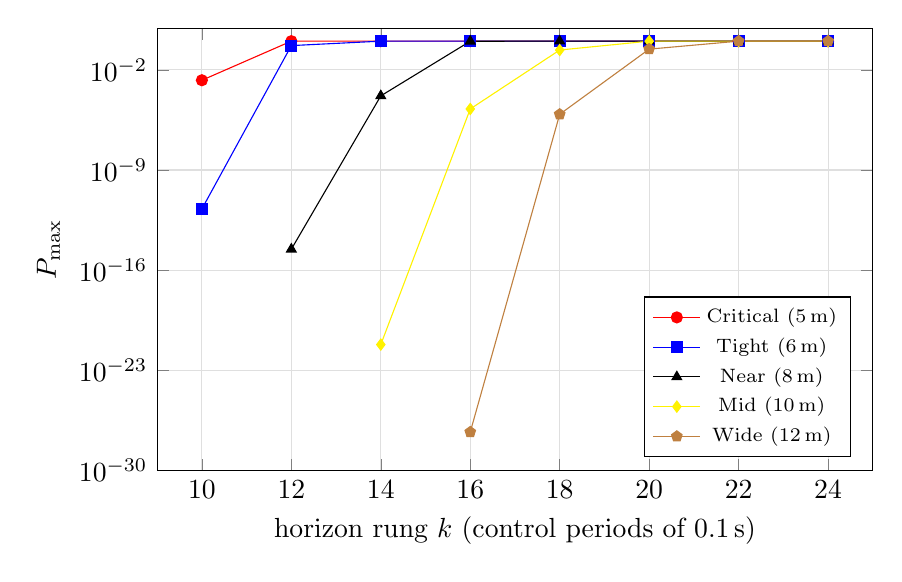
\begin{tikzpicture}
			\begin{semilogyaxis}[
				width=0.88\textwidth, height=7.2cm,
				xlabel={horizon rung $k$ (control periods of $0.1$\,s)},
				ylabel={$P_{\max}$},
				xmin=9, xmax=25, ymin=1e-30, ymax=8,
				xtick={10,12,14,16,18,20,22,24},
				legend pos=south east, legend style={font=\scriptsize},
				grid=both, grid style={gray!25},
				cycle list name=color list]
				\addplot+[mark=*] coordinates {(10,0.001859491711)(12,1)(14,1)(16,1)(18,1)(20,1)(22,1)(24,1)};
				\addlegendentry{Critical ($5$\,m)}
				\addplot+[mark=square*] coordinates {(10,1.90329532e-12)(12,0.4890585366)(14,1)(16,1)(18,1)(20,1)(22,1)(24,1)};
				\addlegendentry{Tight ($6$\,m)}
				\addplot+[mark=triangle*] coordinates {(12,2.923025817e-15)(14,0.0001504356093)(16,0.9893959729)(18,1)(20,1)(22,1)(24,1)};
				\addlegendentry{Near ($8$\,m)}
				\addplot+[mark=diamond*] coordinates {(14,6.379221313e-22)(16,1.834522015e-05)(18,0.239932871)(20,1)(22,1)(24,1)};
				\addlegendentry{Mid ($10$\,m)}
				\addplot+[mark=pentagon*] coordinates {(16,4.951962645e-28)(18,7.815790461e-06)(20,0.2771274783)(22,0.9998060877)(24,1)};
				\addlegendentry{Wide ($12$\,m)}
			\end{semilogyaxis}
		\end{tikzpicture}
		\caption{Worst-case crash probability against the horizon rung for the Following family, logarithmic vertical axis. Each point is one checker result on the certified \code{extra\_fine} encoding; rungs at which $P_{\max}$ is exactly $0$ cannot be drawn on a logarithmic axis and are omitted (Table~\ref{tab:followingresults} records them). The curves shift right with the starting gap without crossing.}
		\label{fig:followingcurves}
	\end{figure}
	
	\begin{figure}[h]
		\centering
		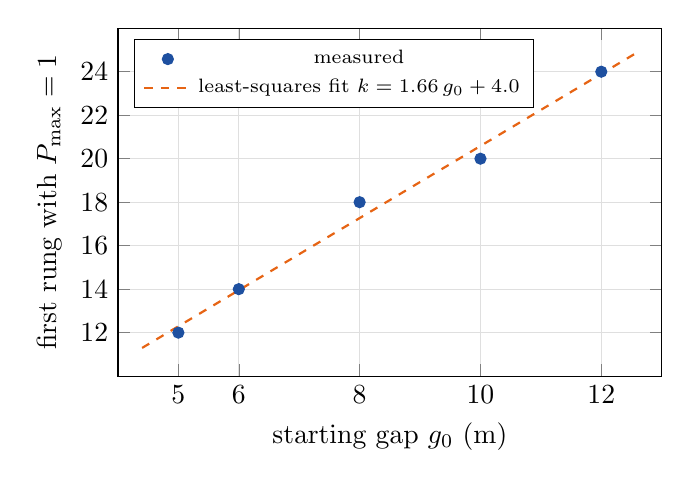
\begin{tikzpicture}
			\begin{axis}[
				width=0.7\textwidth, height=6cm,
				xlabel={starting gap $g_0$ (m)},
				ylabel={first rung with $P_{\max} = 1$},
				xmin=4, xmax=13, ymin=10, ymax=26,
				xtick={5,6,8,10,12}, ytick={12,14,16,18,20,22,24},
				grid=both, grid style={gray!25},
				legend pos=north west, legend style={font=\scriptsize}]
				\addplot[only marks, mark=*, imdpBlue] coordinates {(5,12)(6,14)(8,18)(10,20)(12,24)};
				\addlegendentry{measured}
				\addplot[dashed, thick, accentOrange, domain=4.4:12.6] {1.6585*x + 4.0};
				\addlegendentry{least-squares fit $k = 1.66\,g_0 + 4.0$}
			\end{axis}
		\end{tikzpicture}
		\caption{Saturation rung against starting gap for the Following family. The dashed line is a descriptive least-squares fit, $k \approx 1.66\,g_0 + 4.0$; its reciprocal slope, $0.60$\,m of starting gap per period, is the empirical worst-case closure rate of the certified intervals for this family. The fit is descriptive, not a bound.}
		\label{fig:saturation}
	\end{figure}
	
	\paragraph{Cost.}
	The fine-rung maximise batch ($24$ properties) completed in $3{,}494.9$\,s of wall-clock time at a peak of $30{,}878$\,MB; the coarse batches complete within the resource envelope of Section~\ref{sec:cs:exp}. The window trade of Section~\ref{sec:abs:budget} is thus realised at no increase in verification cost over the production grid.
	
	\paragraph{Simulation corroboration.}
	A Monte Carlo campaign simulates the modelled system directly: the plant equations of Section~\ref{sec:cs:sys}, the controller quantised at cell centres, and the lead-velocity kernel truncated to the grid band and renormalised, matching the certified modelling kernel. A crash is entry into the crash cell slab; departure from the window ends a run as safe, mirroring the sink routing. Each scenario ran $10{,}000$ trajectories to $k = 24$ under a fixed recorded seed; the simulator's controller logic is asserted against the implementation at startup, and the script is preserved with the artifacts. Every empirical crash fraction lies within its certified bracket. The crash counts are zero at every measured rung except Following\_Near, which recorded $2$ crashes in $10{,}000$ by $k = 18$: fraction $2.0 \times 10^{-4}$, Wilson $95\%$ interval $[5.5 \times 10^{-5},\ 7.3 \times 10^{-4}]$. Two readings follow. First, containment is corroborated on sampled trajectories, independently of the exhaustive per-cell test. Second, the campaign measures the one-sidedness of the brackets: at rungs where $P_{\max}$ lies between $0.24$ and $1$, the empirical fractions are at most $2.0 \times 10^{-4}$, with $95\%$ upper confidence limits at most $7.3 \times 10^{-4}$, and at Following\_Critical, $k = 10$, the upper confidence limit $3.8 \times 10^{-4}$ falls below $P_{\max} = 1.86 \times 10^{-3}$ itself. The fractional $P_{\max}$ values therefore quantify the worst case admissible within the certified intervals, not the likelihood of the modelled system; the distance between the two is the one-sidedness identified in Section~\ref{sec:cs:exp} and taken up in Section~\ref{sec:cs:future}.
	
	\subsection{Future work}
	\label{sec:cs:future}
	
	The perfect-perception abstraction is the baseline of the wider programme (Section~\ref{sec:intro}). Track~2 quantifies the perception components into per-input uncertainty tuples; Track~3 replaces the identity perception module of Section~\ref{sec:abs:full} with an enumeration of perception outputs weighted by those tuples, producing the end-to-end model from which runtime monitors are synthesised. The noise state-independence trip-wire of Algorithm~\ref{alg:imagebox} marks exactly the point at which that composition will force the interval computation to range over state-dependent noise. The Following brackets of Section~\ref{sec:cs:extrafine} are the quantitative baseline against which the perception-aware model's brackets will be compared.
	
	Within the present track, two items remain. First, the nondeterministic lead: a lead that chooses per step from a set of admissible accelerations~\cite{EuroNCAP} requires a second action axis in the discretiser and the composition, over which the checker would quantify adversarially; it is defined in the implementation but not composed. Second, the width structure of the brackets. The zero lower bounds are exact for width-preserving deterministic dynamics (Section~\ref{sec:cs:exp}), so every measured $P_{\min}$ in this paper is $0$ and the reported brackets are one-sided: informative upper bounds, trivial lower bounds. Three levers could produce informative lower bounds: abstractions whose transitions target \emph{sets} of states rather than individual cells, which preserve the coherence the per-target intervals discard~\cite{GL25}; game-based abstractions, which separate the abstraction's nondeterminism from the system's and tighten both bounds~\cite{KNP06}; and actuation noise on the ego dynamics, which would make the ego dimension stochastic and remove the straddling indicators that force the zeros, at the price of a second stochastic dimension in the kernel. [UNVERIFIED: the characterisations of \cite{GL25} and \cite{KNP06} are to be checked against the sources before circulation.]
	
	\section{Conclusion}
	\label{sec:concl}
	
	We have documented a partition-based IMDP abstraction pipeline for a stochastic hybrid AEBS model under perfect perception. The construction follows the partition-based framework in its overall architecture and adopts its per-transition range bound on the stochastic dimension~\cite{Soudjani2013}; it departs from that framework by targeting an interval-valued model, by enumerating exact deterministic images through corner evaluation in the style of mixed-monotone reachability~\cite{CA15}, and by certifying soundness through exhaustive per-transition containment under the Markov set-chain preservation result~\cite{DAK12,Hartfiel98} rather than through an additive error bound, which is structurally uninformative here (Sections~\ref{sec:rw}, \ref{sec:abs:sound}). Soundness rests on a single hypothesis, the containment of the modelled kernel's transition probabilities within the stored intervals, and that hypothesis is discharged by test on the shipped artifacts: zero violations across all cells and actions on both certified configurations.
	
	The verification campaigns quantify what the certified models decide. On the production grid, robust model checking certifies a crash probability of exactly $1$ from the imminent-collision scenario, and the horizon-resolved campaign locates the decidable horizon of every other scenario to one rung at five-step spacing, with $P_{\min} = 0$ throughout as the width analysis predicts. The resolution sweep ties the frontier positions to the design rules of Section~\ref{sec:abs:budget}. The second certified configuration then delivers what the production resolution cannot: fractional, scenario-discriminating brackets across the five-state Following family, ordered by starting gap at every measured rung, saturating one metre of gap at a time (Figures~\ref{fig:followingcurves} and~\ref{fig:saturation}). Together the two configurations report a division of labour fixed by the resolution rules: the coarse grid decides the static scenario family over a wide window, and the fine grid carries the fractional results over a narrow one. These brackets are the perfect-perception baseline into which the subsequent tracks of the programme will inject perception-side uncertainty, and against which the end-to-end, monitor-synthesising model will be measured.
	
	\bibliographystyle{plain}
	\bibliography{ref}
	
\end{document}